% !TEX encoding = UTF-8 Unicode

\documentclass[12pt,a4j,titlepage]{ltjsarticle}
\usepackage{semi}
\usepackage{here}
\usepackage{listings} % listingを使うため

\lstset{
 	breaklines = true,
 	breakindent = 10pt,
 	classoffset = 0,
 	keywordstyle = {\bfseries \color[cmyk]{0,1,0,0}},
 	frame = single,
 	framesep = 5pt,
 	numbers = left,
 	stepnumber = 1,
 	tabsize = 4,
 	captionpos = t
}

% \title{}
% \author{}
% \date{}

\begin{document}

\begin{titlepage}
  \begin{center}
  
    \vspace*{20truept}
    
    {\LARGE 2022年度 卒業論文} 
    
    \vspace*{75truept}
    
    {\Huge } %論文タイトル
    
    \vspace{10truept}
    {\LARGE 楽曲のミックスダウンにおけるエフェクターによる}

    {\Huge } %論文タイトル 長い場合 改行1

    {\LARGE 効果と変化を理解するためのシミュレータ教材}
    \vspace{10truept}

    {\Huge } %論文タイトル 改行2
    
    \vspace{85truept}
    
    {\LARGE 指導教員 須田 宇宙 准教授}
    
    \vspace{60truept}
    
    {\LARGE 千葉工業大学 情報ネットワーク学科}
    
    \vspace{15truept}
    
    {\LARGE 須田研究室}
    
    \vspace{70truept}
    
    {\LARGE 1932148 氏名 依田 樹 } % 氏名は消さない 学生番号 氏名 名前

    \vspace{70truept}
    
  \end{center}
  \begin{flushright}

    {\LARGE 提出日 2023年1月17日}
  
  \end{flushright}
\end{titlepage}

\pagenumbering{roman}
\setcounter{tocdepth}{3}
% 目次の出力
\tableofcontents
\newpage
% 表目次
\listoftables
% 図目次
\listoffigures
\clearpage
\pagenumbering{arabic}
\setcounter{page}{1}
\section{緒言}
音楽制作には, メロディを作る「作曲」,歌詞を書く「作詞」,楽器の音を選択して伴奏を作る「編曲」などのほかに,複数の音源をエフェクターを用いて整え一つにする「ミックスダウン」という工程がある\cite{mix}.
近年は,コンピュータ上で音楽制作ができるDTMと呼ばれるものが普及して手軽に音楽制作ができるようになった.
それにより,作曲から編曲,ミックスダウンまで一人で完結させることも多くなっている.
また,近年のデジタル化により,機材がハードウェアからソフトウェアになり,ミックスダウンも費用をかけずに誰でも挑戦することができるようになった\cite{digital}.

しかし,ミックスダウンは,作曲,作詞,編曲に比べ,変化が分かりにくく,非常に学びづらい.
また, ミックスダウンの経験が少なく,エフェクターを使いこなせない人にとってが説明だけではわからないという問題点がある。

そこで本研究では, 実際に操作し, 各エフェクターの使い方やその効果を知るためのシミュレータ教材を開発することを目的とする.

\newpage
\section{音楽制作について}
\subsection{音楽の歴史}
音楽のはっきりとした起源は定かではないが,記録として残されているものとして最古のものはメソポタミア音楽であり,楽器を演奏している人々の姿が刻まれたレリーフが発見されている.
音楽は紀元前の間では,儀式や祭りで使われ,音楽やリズムが体系づけられていった.
5\sim15世紀は,キリスト教がかかわり,教会で歌われることになり,楽譜を使い,正確に音の高さを表すようにもなった.
17\sim18世紀では,バロック音楽というものが流行し,形式ばった音楽から自由な表現をする音楽が増えてきた.
18\sim19世紀では,弦楽四重奏や協奏曲などが登場し,一般市民も聞くことができるようになった.
19\sim20世紀では,無調の音楽や十二音音楽も登場や電子音楽の登場により,様々なジャンルが確立された\cite{history}.

\subsection{DTM}
DTMは,Desk Top Musicの略称であり,主にコンピュータを使った音楽制作のことをいう.
実際に楽器を演奏できなくても,マウスで音を並べていき,音楽を作ることができる.
また,楽器ができる人は,簡単に録音することや編集することなどができる\cite{dtm}.

コンピュータで音楽制作をするためのソフトウェアをDigital Audio Workstation(DAW)といい,DTMをするにはDAWが必要となる.
DAWでは,オーディオの録音,編集やMIDIデータの編集などができ,作曲や編曲,ミックスダウンができる\cite{daw}.

\subsubsection{ソフトウェア音源}
MIDIを操作して音を出し楽曲を制作するには,ソフトウェア音源が必要である.
ソフトウェア音源は,単体のハード機器のシンセサイザーをソフトウェアで再現したものである\cite{software}.
ソフトウェア音源はDAWに付属されていることが多いが,よりリアルな音を出すためや,出したい音色を出すためには有料で別途,ソフトウェア音源を買うことが必要である.

\subsubsection{プラグインエフェクター}
ミックスダウンをするには,プラグインエフェクターが必要である.
プラグインエフェクターは,アナログのエフェクターをデジタルで再現したものである.
プラグインエフェクターはソフトウェア音源と同じくDAWに付属されていることが多いが,より高度な処理をするためや,自分の使いやすいUIのものを使うためには有料で別途,プラグインエフェクターを買うことが必要である.

\subsection{ミックスダウン}
録音された複数の音源に音色を整えるためのエフェクターで効果を与えて聞きやすくし,それらをまとめて一つの楽曲に仕上げることをミックスダウンという.
ミックスダウンの概念図を図\ref{fig:gainen}に示す.
左側にそれぞれの楽器の録音された音源があり,左から順番にエフェクターの効果を与え最終的にすべてをまとめて一つの楽曲の音源として完成させる.
またある特定の楽器同士をまとめてそれらにエフェクターで効果を与える場合もある.
例えば,図\ref{fig:gainen}では,バスドラム,スネアドラム,ハイハットをドラムとしてまとめて,それらにコンプレッサーを与えるという作業をしている.

\begin{figure}[H]
\centering
 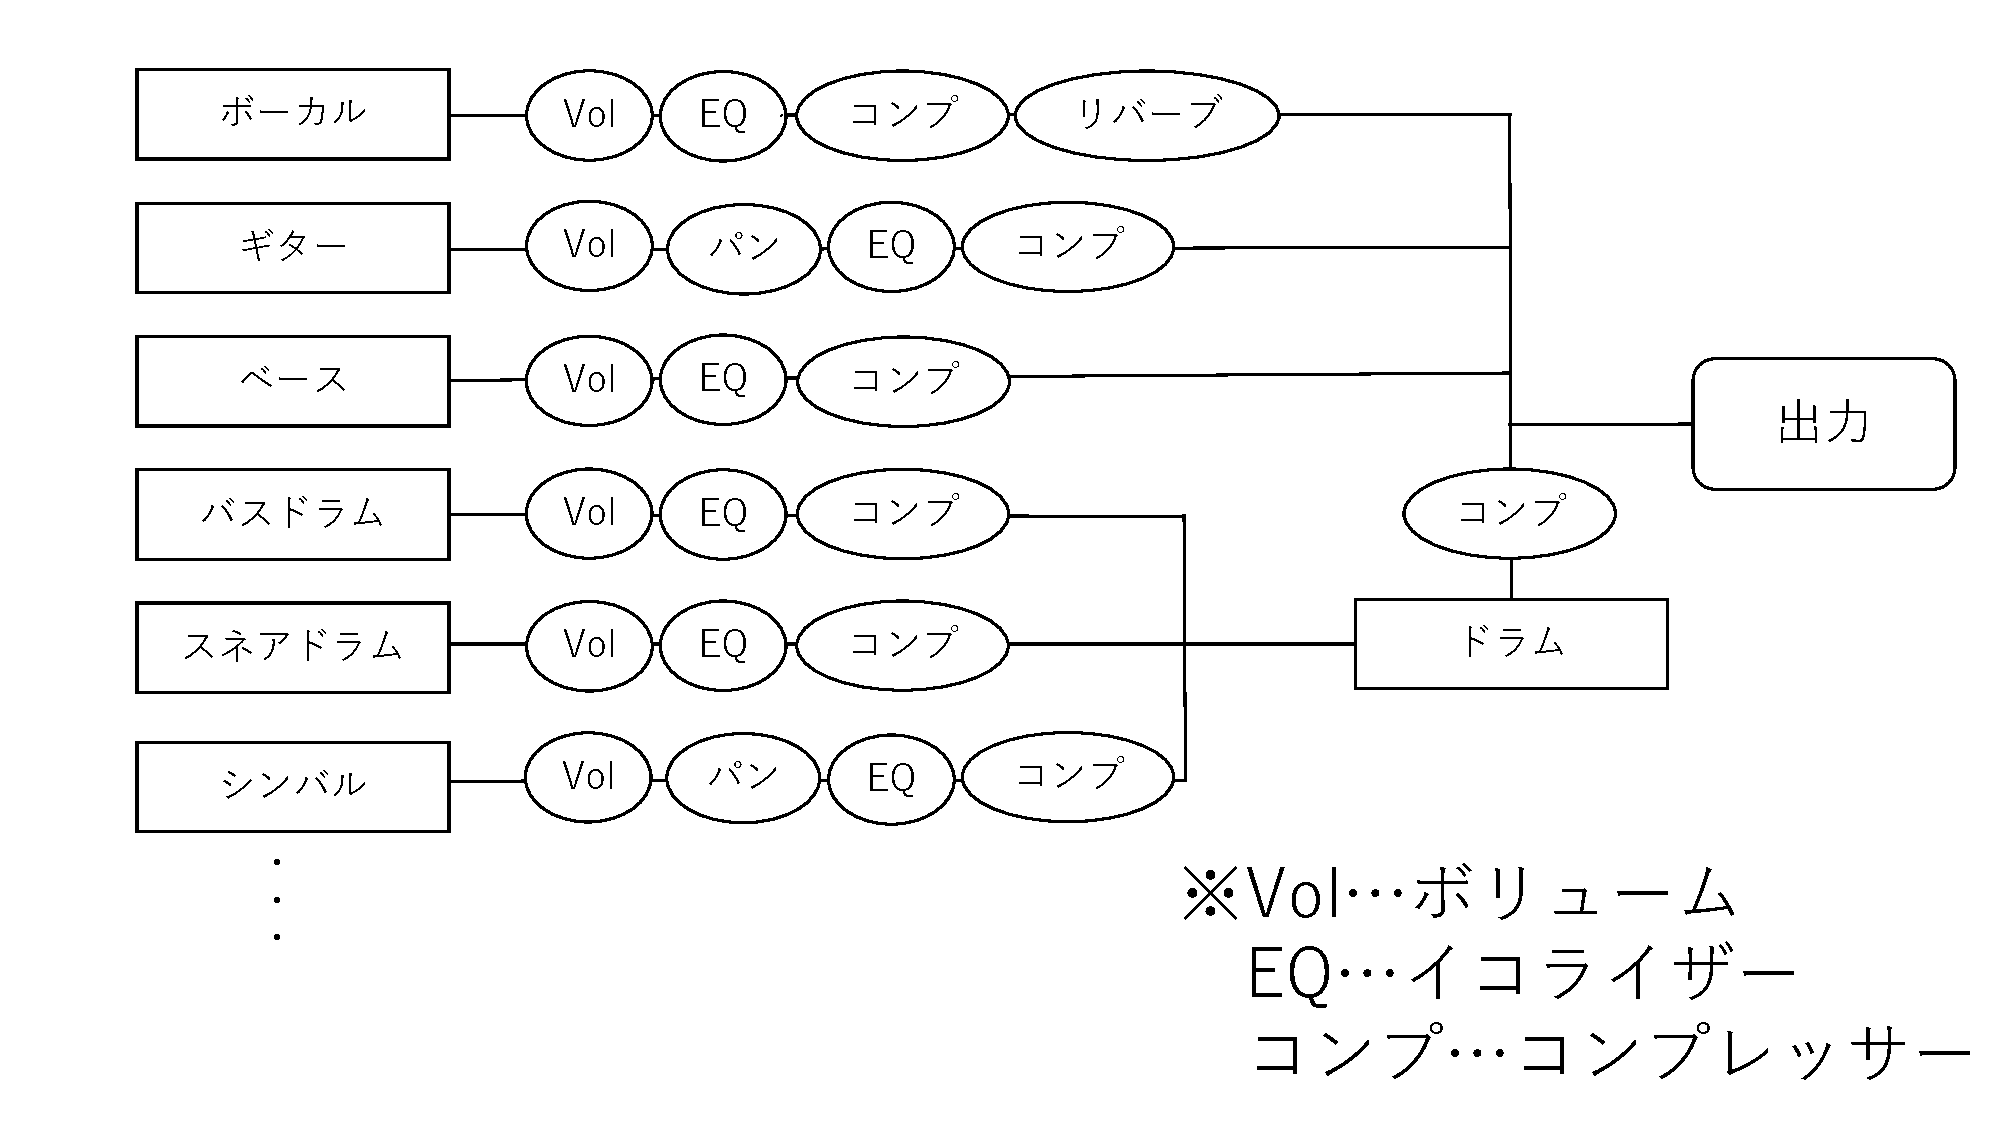
\includegraphics[width=120mm]{./figures/gainen.pdf}
 \caption{ミックスダウンの概念図}
 \label{fig:gainen}
\end{figure}

エフェクターでの効果の与え方にはインサート,センドという2種類がある.
インサートは,音源に直接エフェクターを繋ぎ,効果を与える方法である.
基本的には,エフェクターはインサートで与えることが多い.
センドは,音源と同じ音を別のトラックにもう一つ出力し,その出力した音にエフェクターを繋ぎ,効果を与える方法である.
センドのイメージ図を図\ref{fig:send1}に示す.
図の左にボーカルがあり,それにインサートでイコライザー,コンプレッサー,ディレイで効果を与えている.
そして,ボーカルをセンドでもう一つ音を出力し,リバーブで効果を与えている.
センドは,リバーブとディレイに使われることが多い.
例えば,図\ref{fig:send1}のように,ディレイはインサートで効果を与え,センドでリバーブを与えるとする.
もし,インサートでディレイの後にリバーブを与えるとすると,ディレイでやまびこが追加された音にリバーブで反響音を追加してしまうと音が濁ってしまう.
このような状態を回避するためにセンドを使う場合がある.

\begin{figure}[H]
\centering
 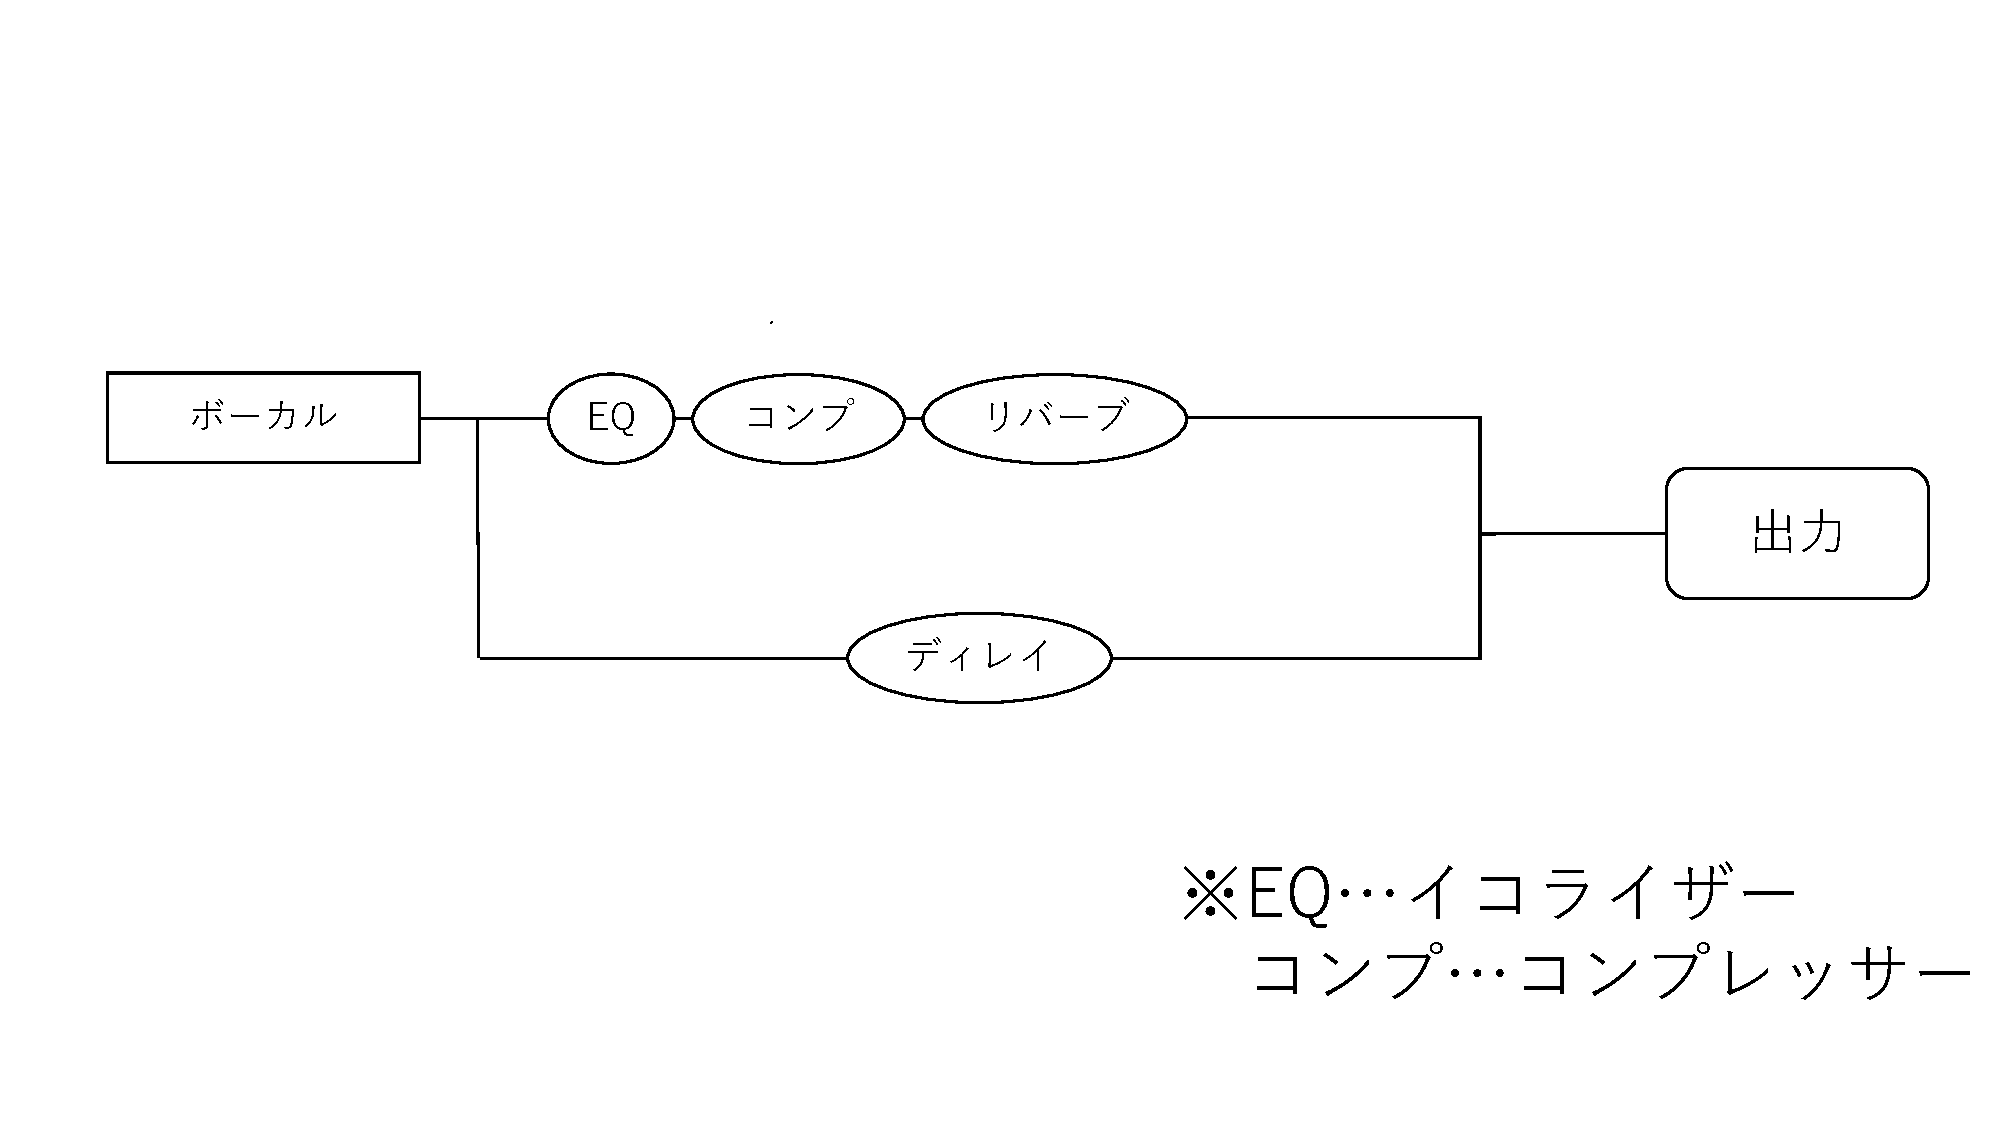
\includegraphics[width=120mm]{./figures/send1.pdf}
 \caption{センドのイメージ図}
 \label{fig:send1}
\end{figure}

また,DTMでミックスダウンをする場合,リバーブやディレイなどの空間系のエフェクターは,高負荷で動作が重くなるということがあり,それを回避するためにセンドを使うことがある.
その場合のイメージ図を図\ref{fig:send2}に示す.
図の左に録音されたボーカルとハモリ1とハモリ2の音源がある.
ボーカルはそのままインサートでイコライザー,コンプレッサー,リバーブが与えられている.
ハモリ1とハモリ2はインサートでイコライザー,コンプレッサーを与え,センドで2つとも同じトラックに出力し,まとめてリバーブを与えている.
このように複数の音源の音をまとめてセンドで出力し,まとめて効果を与えることで,それぞれにリバーブを与えてあげるよりも負荷が軽くなるといったメリットもある.

\begin{figure}[H]
\centering
 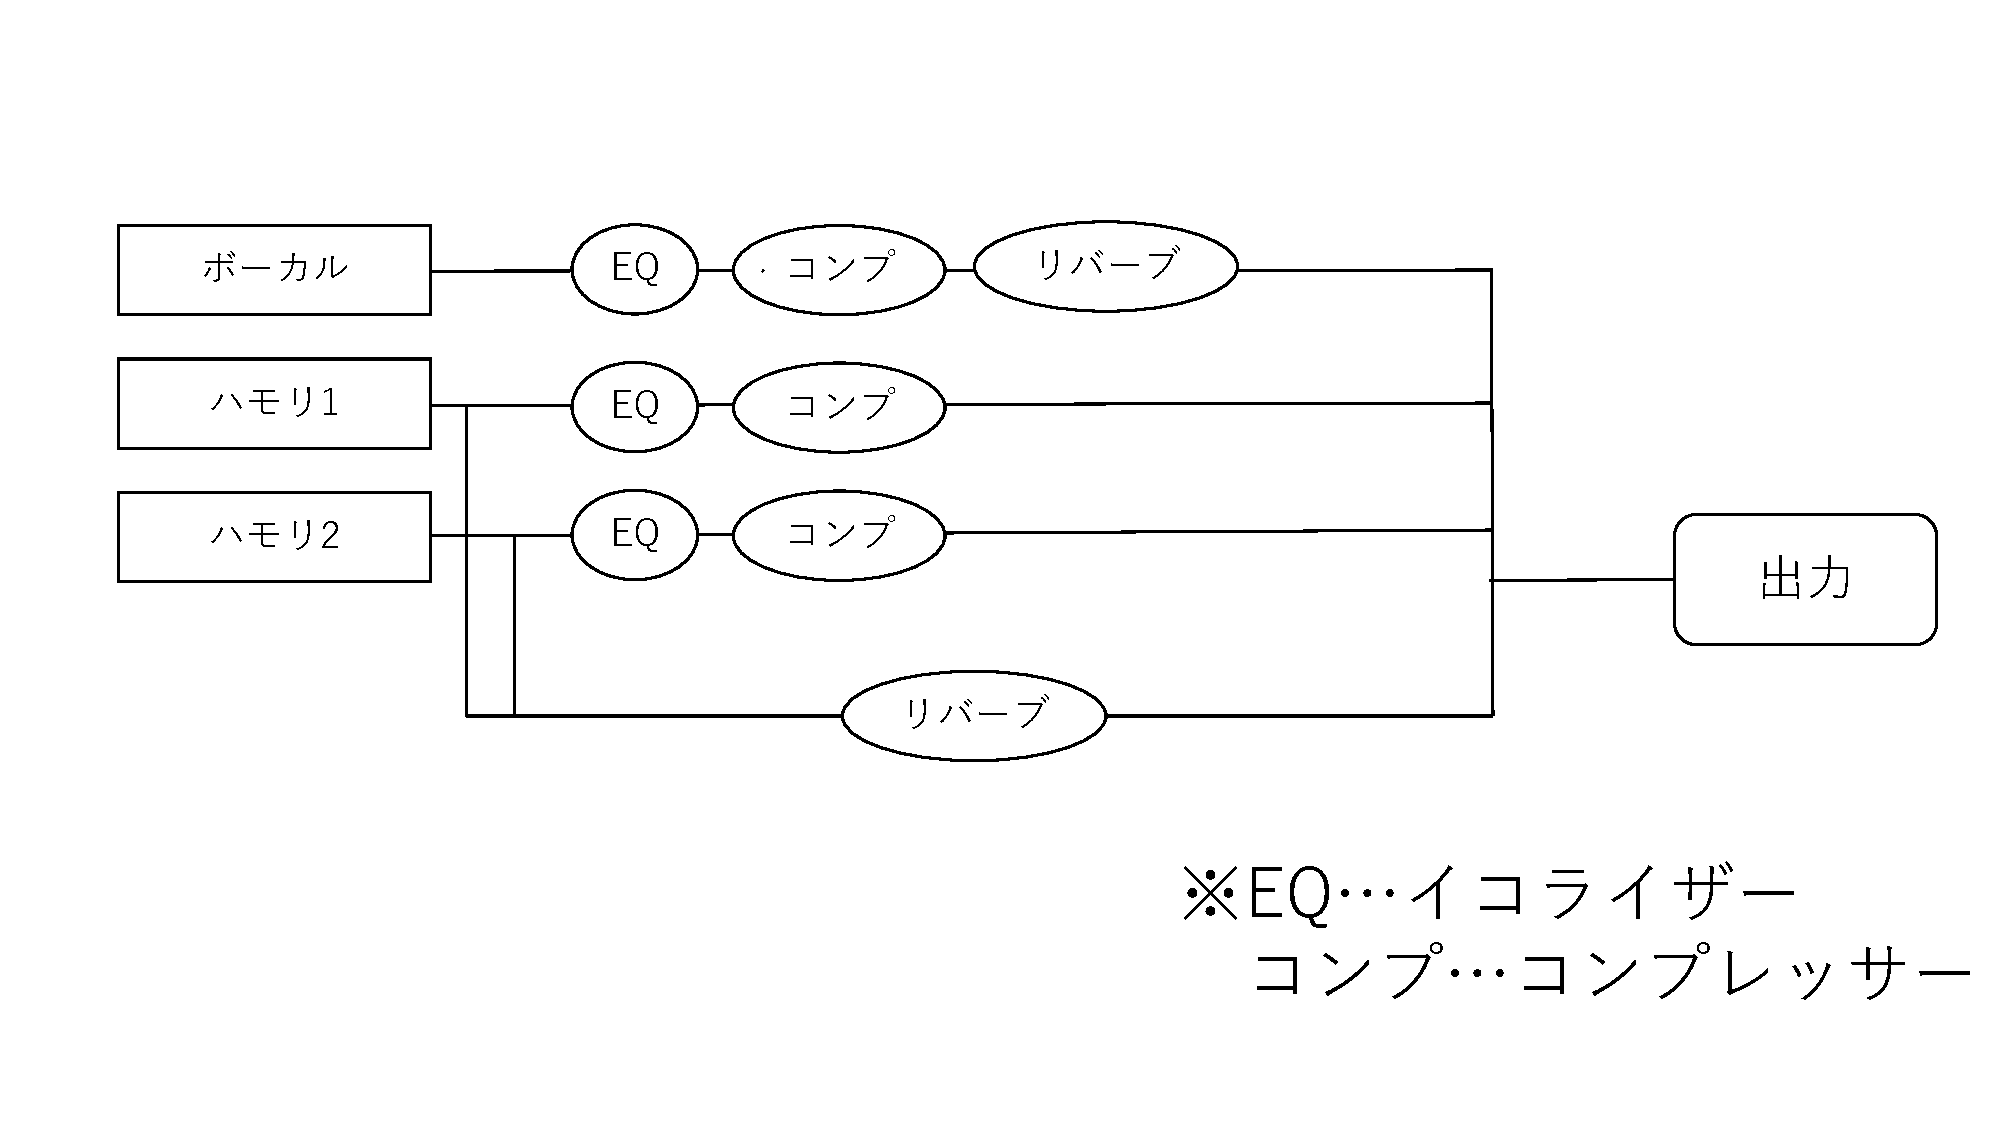
\includegraphics[width=120mm]{./figures/send2.pdf}
 \caption{センドでの高負荷回避@ハモリをセンドで送りまとめてリバーブを与えることで負荷を軽くする}
 \label{fig:send2}
\end{figure}

\newpage
\section{エフェクターについて}
この章では,主にミックスダウンで使われるエフェクターについて説明する.
\subsection{ボリューム}
ボリュームは,音量を調整するエフェクターである.
ミックスダウンにおいては,音量バランスが少し変わるだけでも曲の印象が大きく変わってしまうため、各楽器の音量のバランスを整えて聞きやすくするための重要なエフェクターとなる.
\subsection{パン}
パンは,ステレオの音源で,左右のどの位置から鳴らすかを調整するエフェクターである.ミックスダウンにおいてのパンは,左右でどの位置に楽器が配置されているのかを再現するという効果がある.
実際にライブなどで演奏される楽器の配置にしたがって音源が配置されることが多い.

例えば,ある曲にボーカル,ドラム,ピアノ,ギター,ベースが使われるとする.
担当する位置を大まかに分けると,中央にベース,少し右にピアノ,左右にギター,中央にボーカル,左右と中央にドラムとなる.

\subsection{イコライザー}
イコライザーは,周波数ごとに音量を調整するエフェクターである.
ミックスダウンにおいてのイコライザーは,それぞれの楽器の周波数帯での住み分けに使われる.
具体的な使い方は,その音源の無駄な周波数を下げることや,聞かせたい音源を邪魔しないように,他の楽器の,その聞かせたい音源の芯となる周波数帯を下げることになります.

周波数帯での住み分けについて説明する.
例えば,ある曲にボーカル,ドラム,ピアノ,ギター,ベースが使われるとする.
担当する音域を大まかに分けると,低音域にベース,低音域から高音域にかけてピアノ,中音域にギター,中音域から高音域にかけてボーカル,低音域から高音域にかけてドラムとなる.
それら楽器の範囲にない周波数,例えば,ベースは中音域から高音域,ギターは低音域と高音域のように下げることで住み分けができる.

聞かせたい音源の芯となる周波数帯を下げることについて説明する.
同じように,ある曲にボーカル,ドラム,ピアノ,ギター,ベースが使われるとする.
この曲ではボーカルが目立たせたい楽器とする.
処理前を図\ref{fig:EQ1},処理後を図\ref{fig:EQ2}に示す.
縦軸が音量,横軸が周波数を表す.
黒がドラム,緑がピアノ,黄がギター,赤がボーカルを表す,
ボーカルの芯となる周波数帯と重なる楽器がドラム,ピアノ,ギターとなる.
図\ref{fig:EQ1}のように,処理前はボーカルの芯となる周波数は他の楽器が重なり聞こえにくくなっている.
図\ref{fig:EQ2}のように,ボーカル以外の楽器のボーカルの芯となる周波数を下げてあげてボーカルの入る隙間を作ってあげることで,ボーカルを目立たせることができる.

\begin{figure}[H]
  \begin{minipage}[b]{0.5\linewidth}
    \centering
    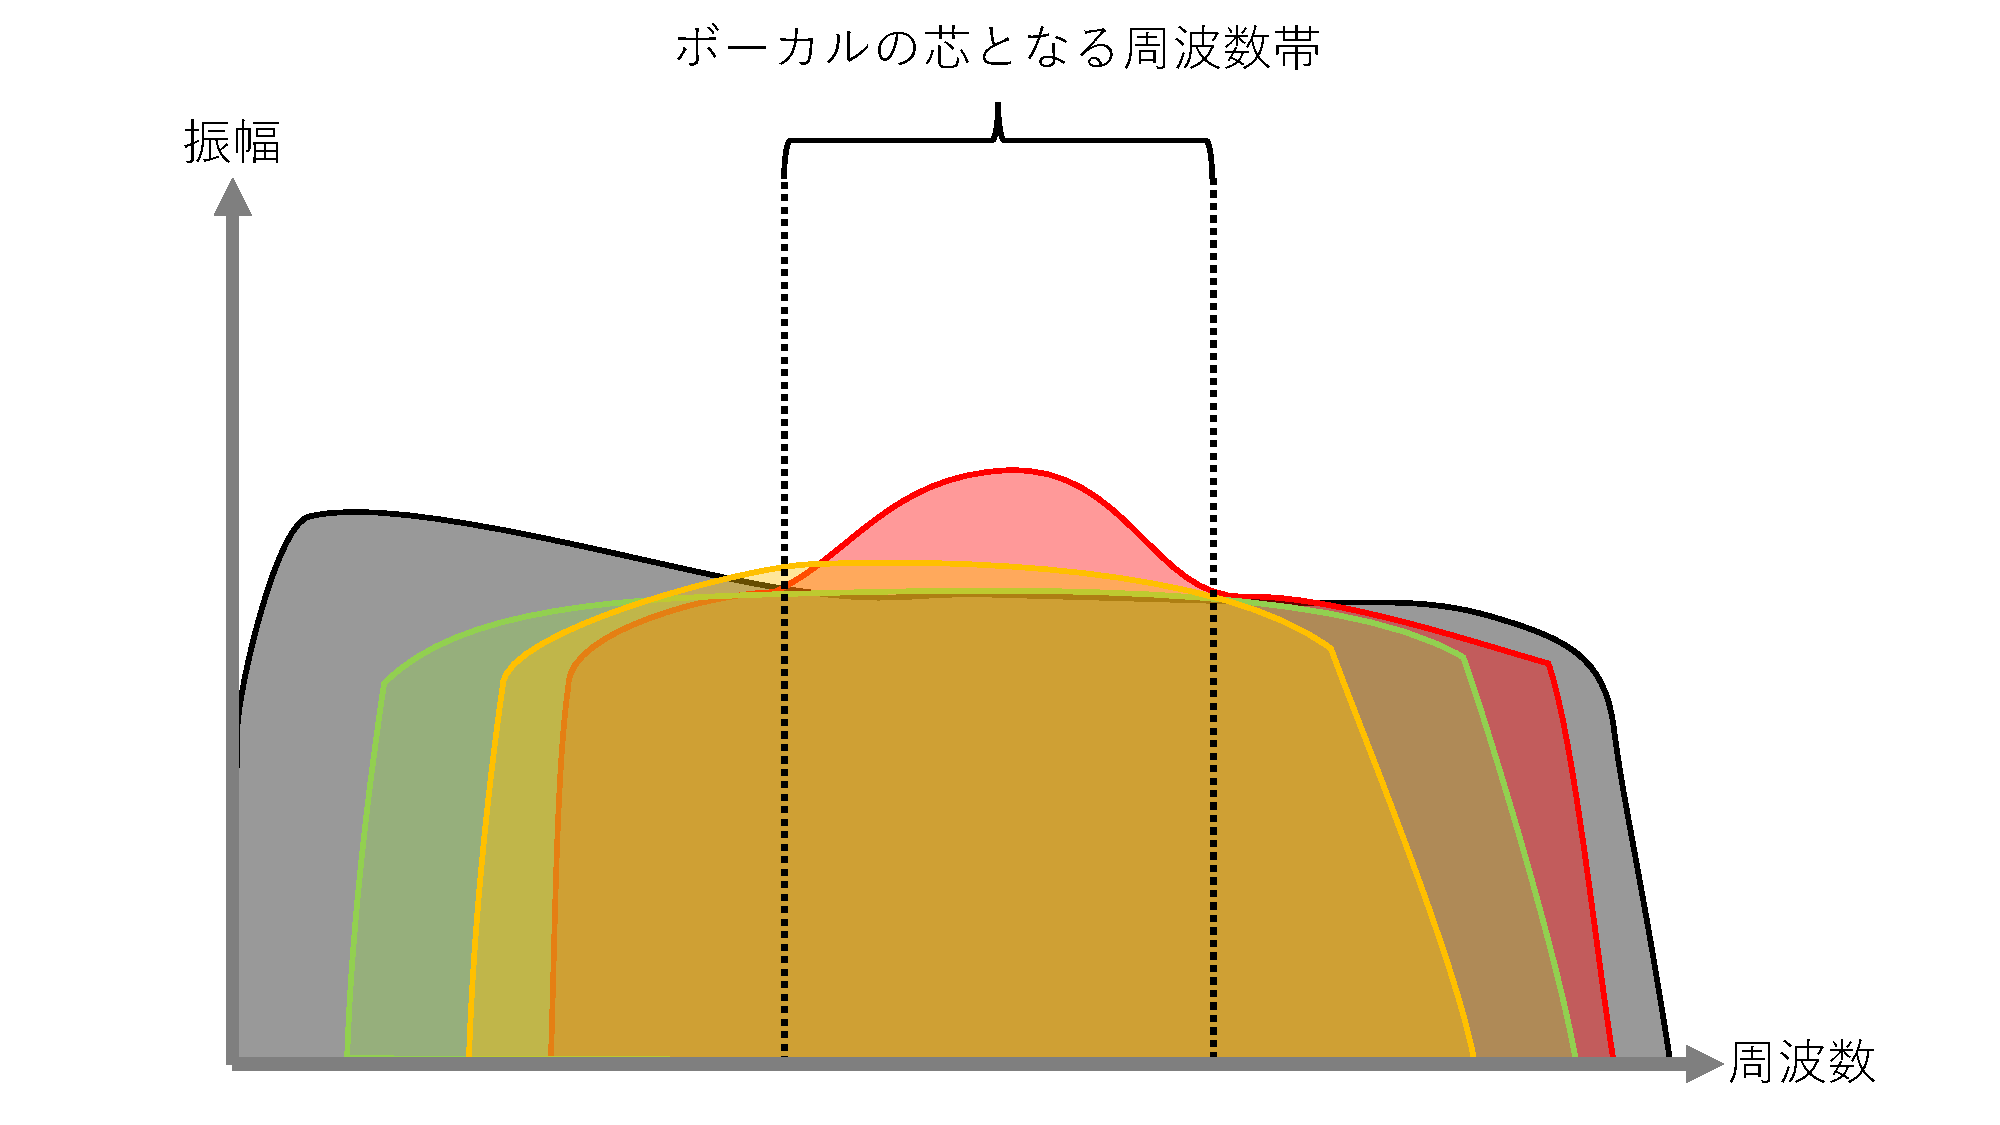
\includegraphics[width=90mm]{./figures/EQ1.pdf}
    \caption{イコライザー処理前@ボーカルの芯となる周波数にその他の楽器が重なってボーカルが聞こえづらい状態}
    \label{fig:EQ1}
  \end{minipage}
  \begin{minipage}[b]{0.5\linewidth}
    \centering
    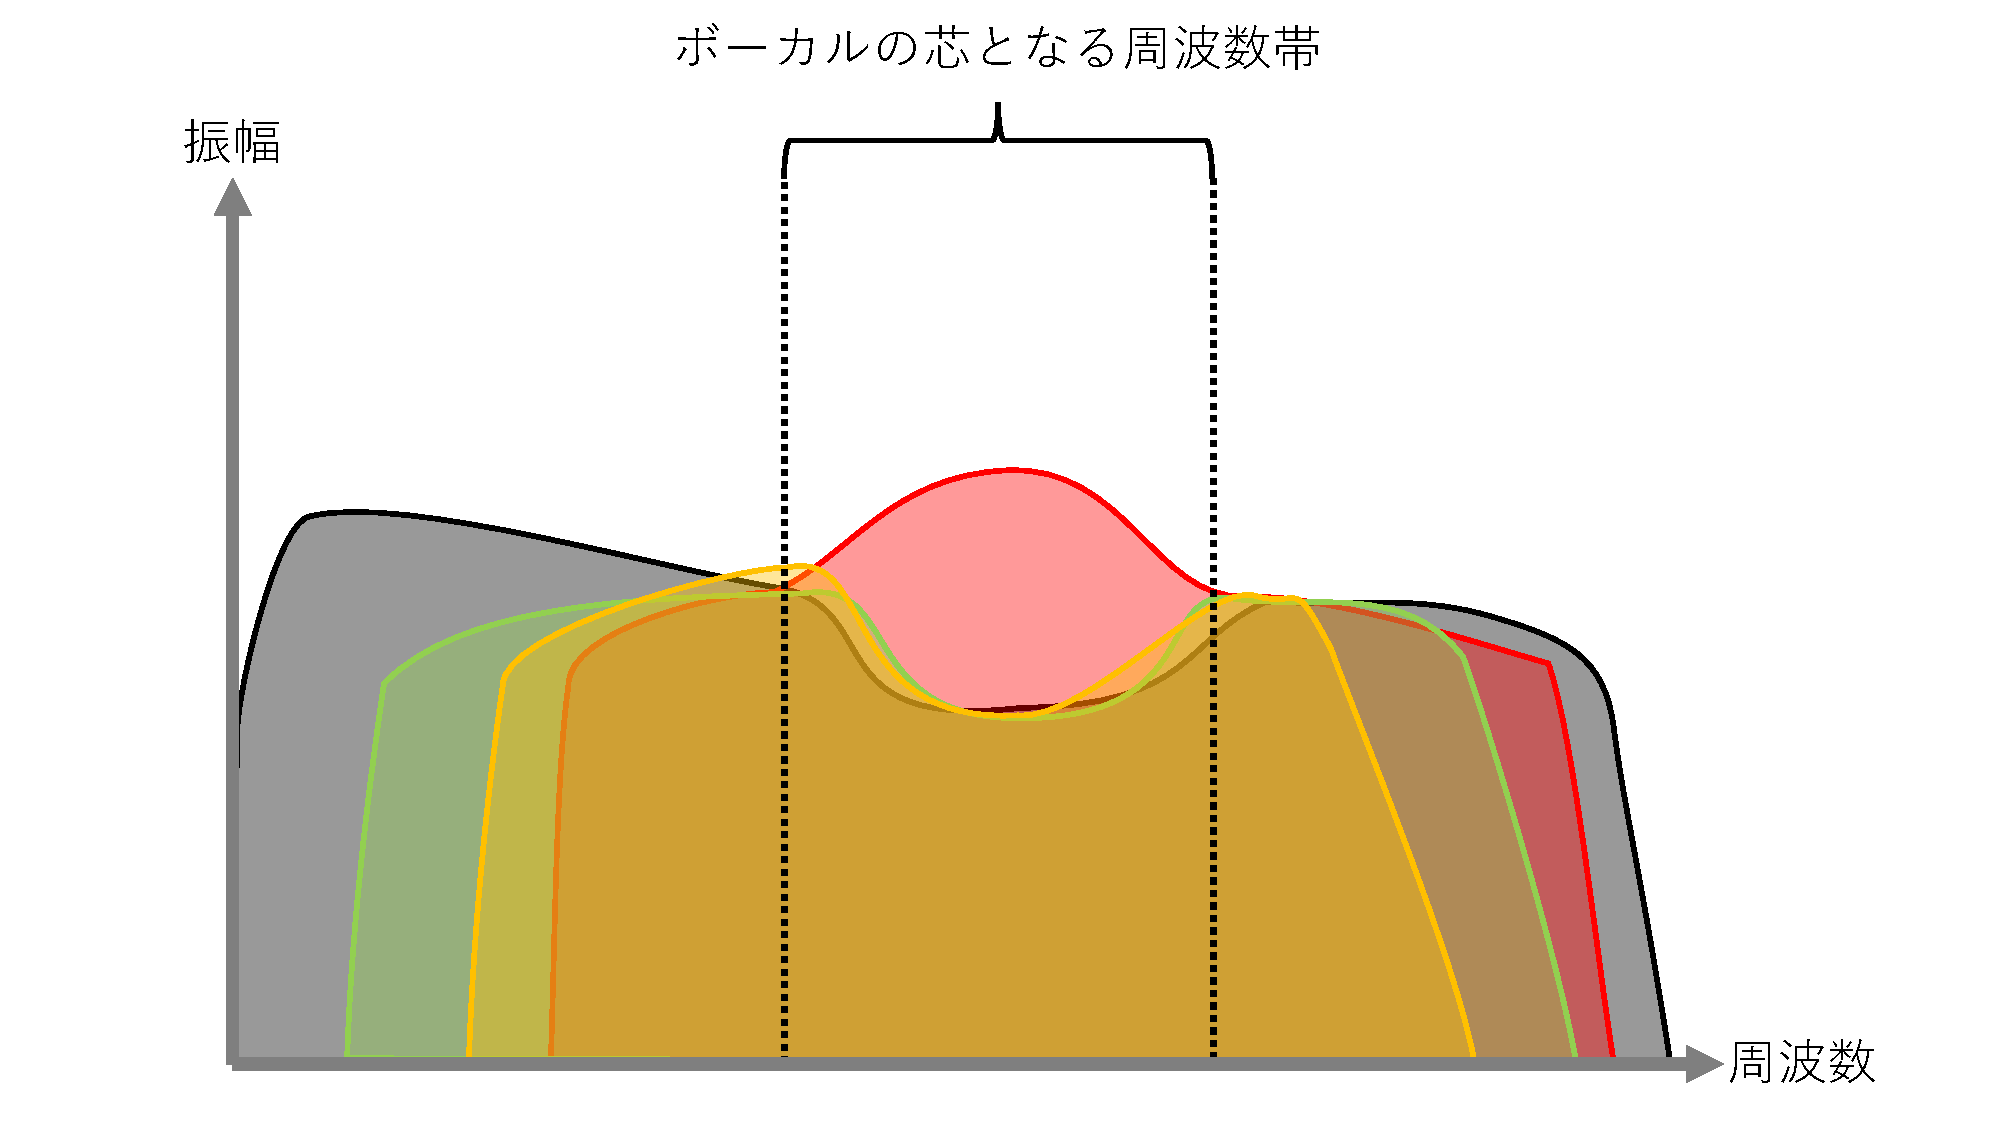
\includegraphics[width=90mm]{./figures/EQ2.pdf}
    \caption{イコライザー処理後@その他の楽器のボーカルの芯となる周波数を削ってボーカルが聞こえやすい状態}
    \label{fig:EQ2}
  \end{minipage}
\end{figure}

\subsection{コンプレッサー}
コンプレッサーは,一定の音量を超えたところを小さくして音量のバラつきをなくすエフェクターである.
ミックスダウンにおいてのコンプレッサーは,音量のバラつきをなくし,音圧をあげるために使われる.

コンプレッサーのパラメーターには主に,スレショルド,レシオ,アタック,リリースなどがある.
スレショルドとレシオを図\ref{fig:comp1}を用いて説明する.
横軸が入力音量で,縦軸が出力音量である.

スレショルドは,音量の圧縮し始める閾値である.図\ref{fig:comp1}の青線がスレショルドを表しており,これ以上の音量になると圧縮が始まる.

レシオは,音量がスレショルドを超えたときに,どの程度圧縮するかの割合を決める値である.
図\ref{fig:comp1}の赤線はスレショルドより大きい音量を表していて,それをどの程度圧縮するかの割合がレシオを表している.
例えば図\ref{fig:comp1}の場合,レシオが1/2に設定されており,赤い線の1/2まで音量を圧縮することとなる.

アタックは,音量がスレショルドを超えた時にどの程度遅れてレシオに到達するかの時間である.
アタック感が大事なドラムなどでは,アタックを遅くすることでアタック感を潰すことなく音量を下げることができる.
アタック感を必要としないギターやシンセサイザーなどでは,アタックを早くすることで,しっかりと音量差を無くし,音圧をあげることができる.

リリースは,音量がスレショルドを下回った時にどの程度遅れて圧縮をやめるかの時間である.
しっかりと抑揚を出したい場合はリリースを長めにして,ある程度抑揚をつけたい場合はリリースを短めにする.

\begin{figure}[H]
\centering
 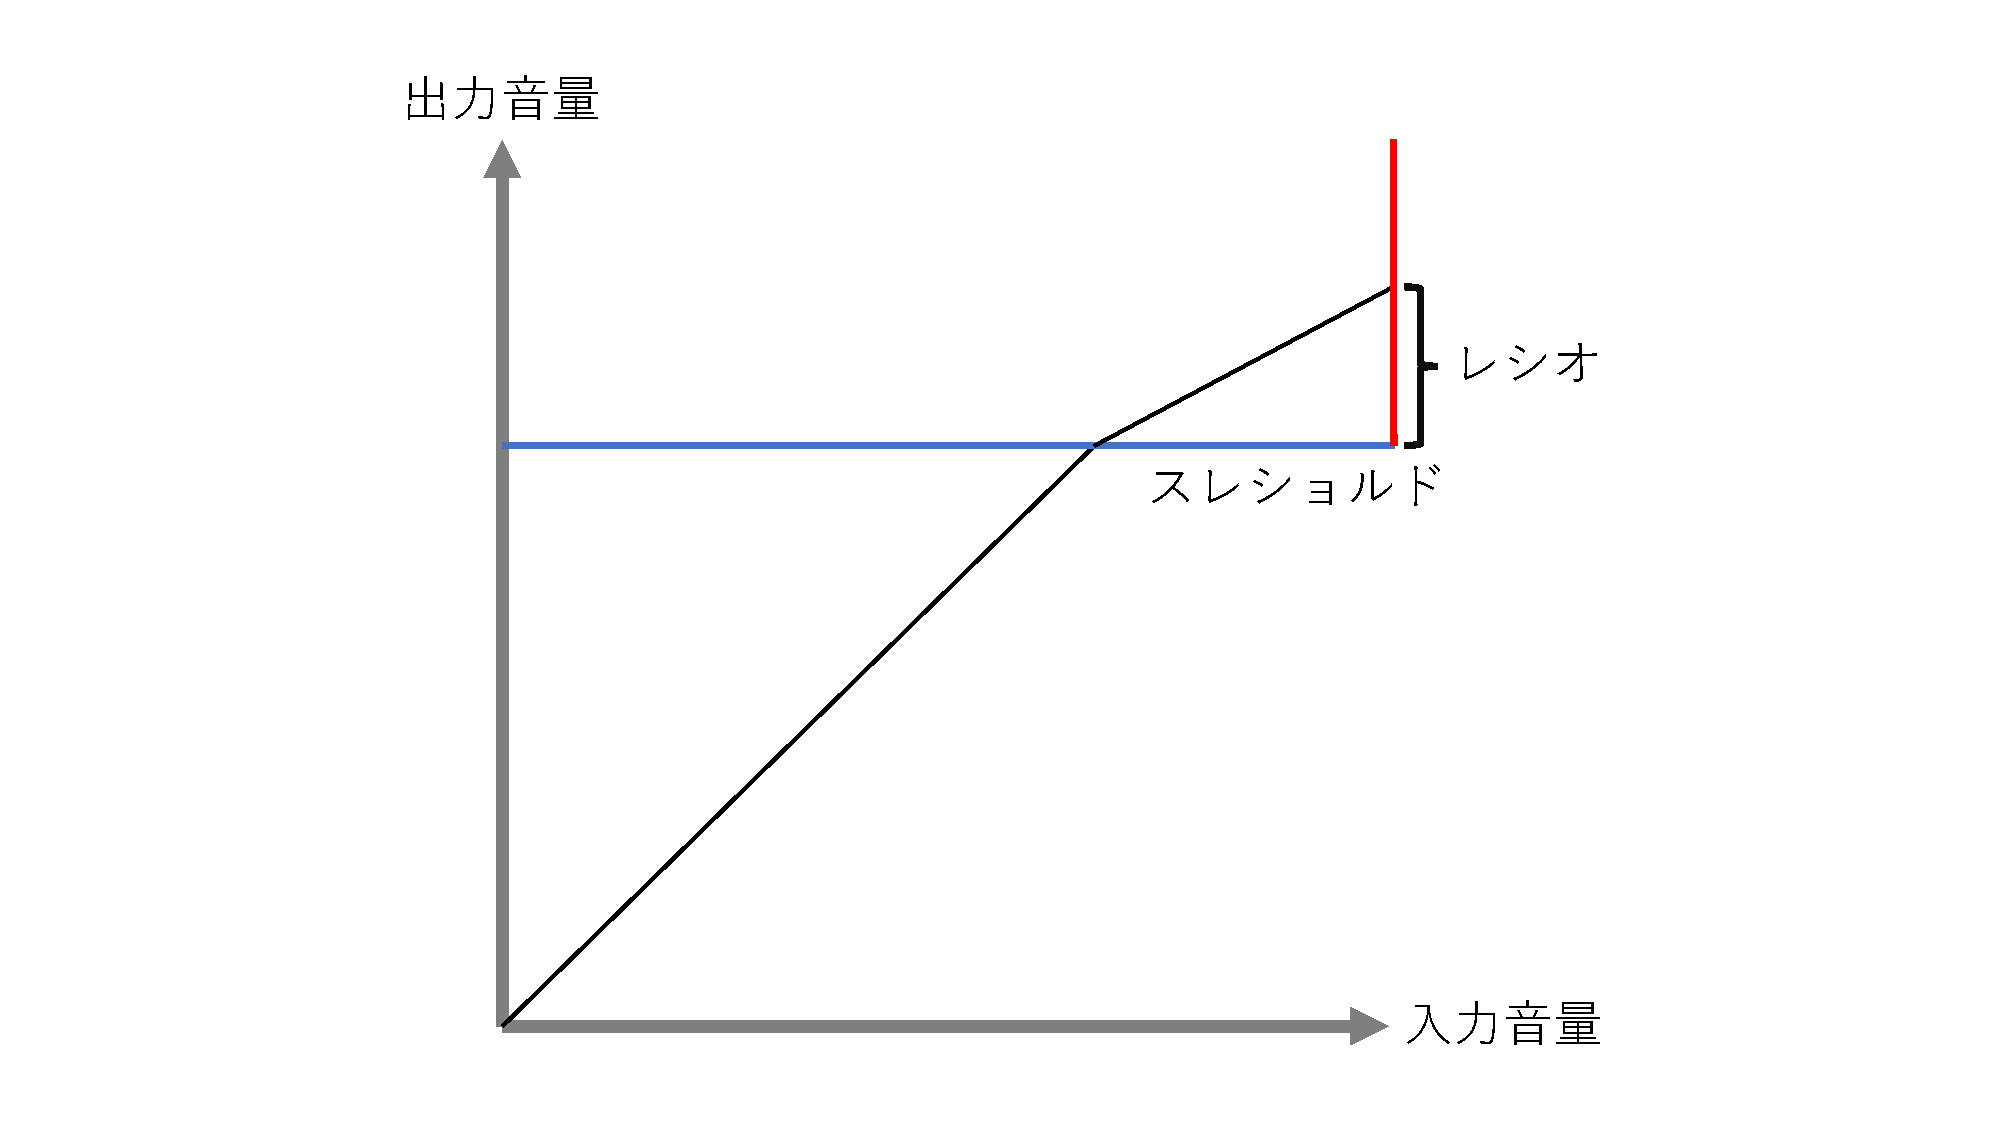
\includegraphics[width=150mm]{./figures/comp1.pdf}
 \caption{スレショルドとレシオ}
 \label{fig:comp1}
\end{figure}

\subsection{ディレイ}
ディレイは,やまびこのように音源から出ている音が遅れて聞こえてくる効果を追加するエフェクターである.
ミックスダウンにおいてのディレイは,隙間を埋めるためや,空間の広さを演出するために使われる.

ディレイのパラメーターには主に,ディレイタイム,フィードバックなどがある.
ディレイタイムとフィードバックを図\ref{fig:delay}を用いて説明する.
横軸が時間で,縦軸が振幅である.
青色の音声波形が原音,黄色の音声波形はディレイで返ってきた音を表している.

ディレイタイムは,ディレイの遅れて聞こえてくる時間で,図\ref{fig:delay}の赤矢印がディレイタイムを表している.
隙間を埋めるために使われるディレイは,ディレイタイムを遅くして使い,空間の広さを演出するために使われるディレイはディレイタイムを早くして使う.

フィードバックは,どの程度の音量で返すかの値で,図\ref{fig:delay}の青矢印がフィードバックを表している.
フィードバックは,曲のジャンルや曲の中の展開でも値が変わってくる.例えば,激しい曲調の曲ではフィードバックの値を大きくして迫力を出すことや,静かな曲調ではフィードバックの値を小さくして,やわらかい雰囲気を出すなどできる.

\begin{figure}[H]
\centering
 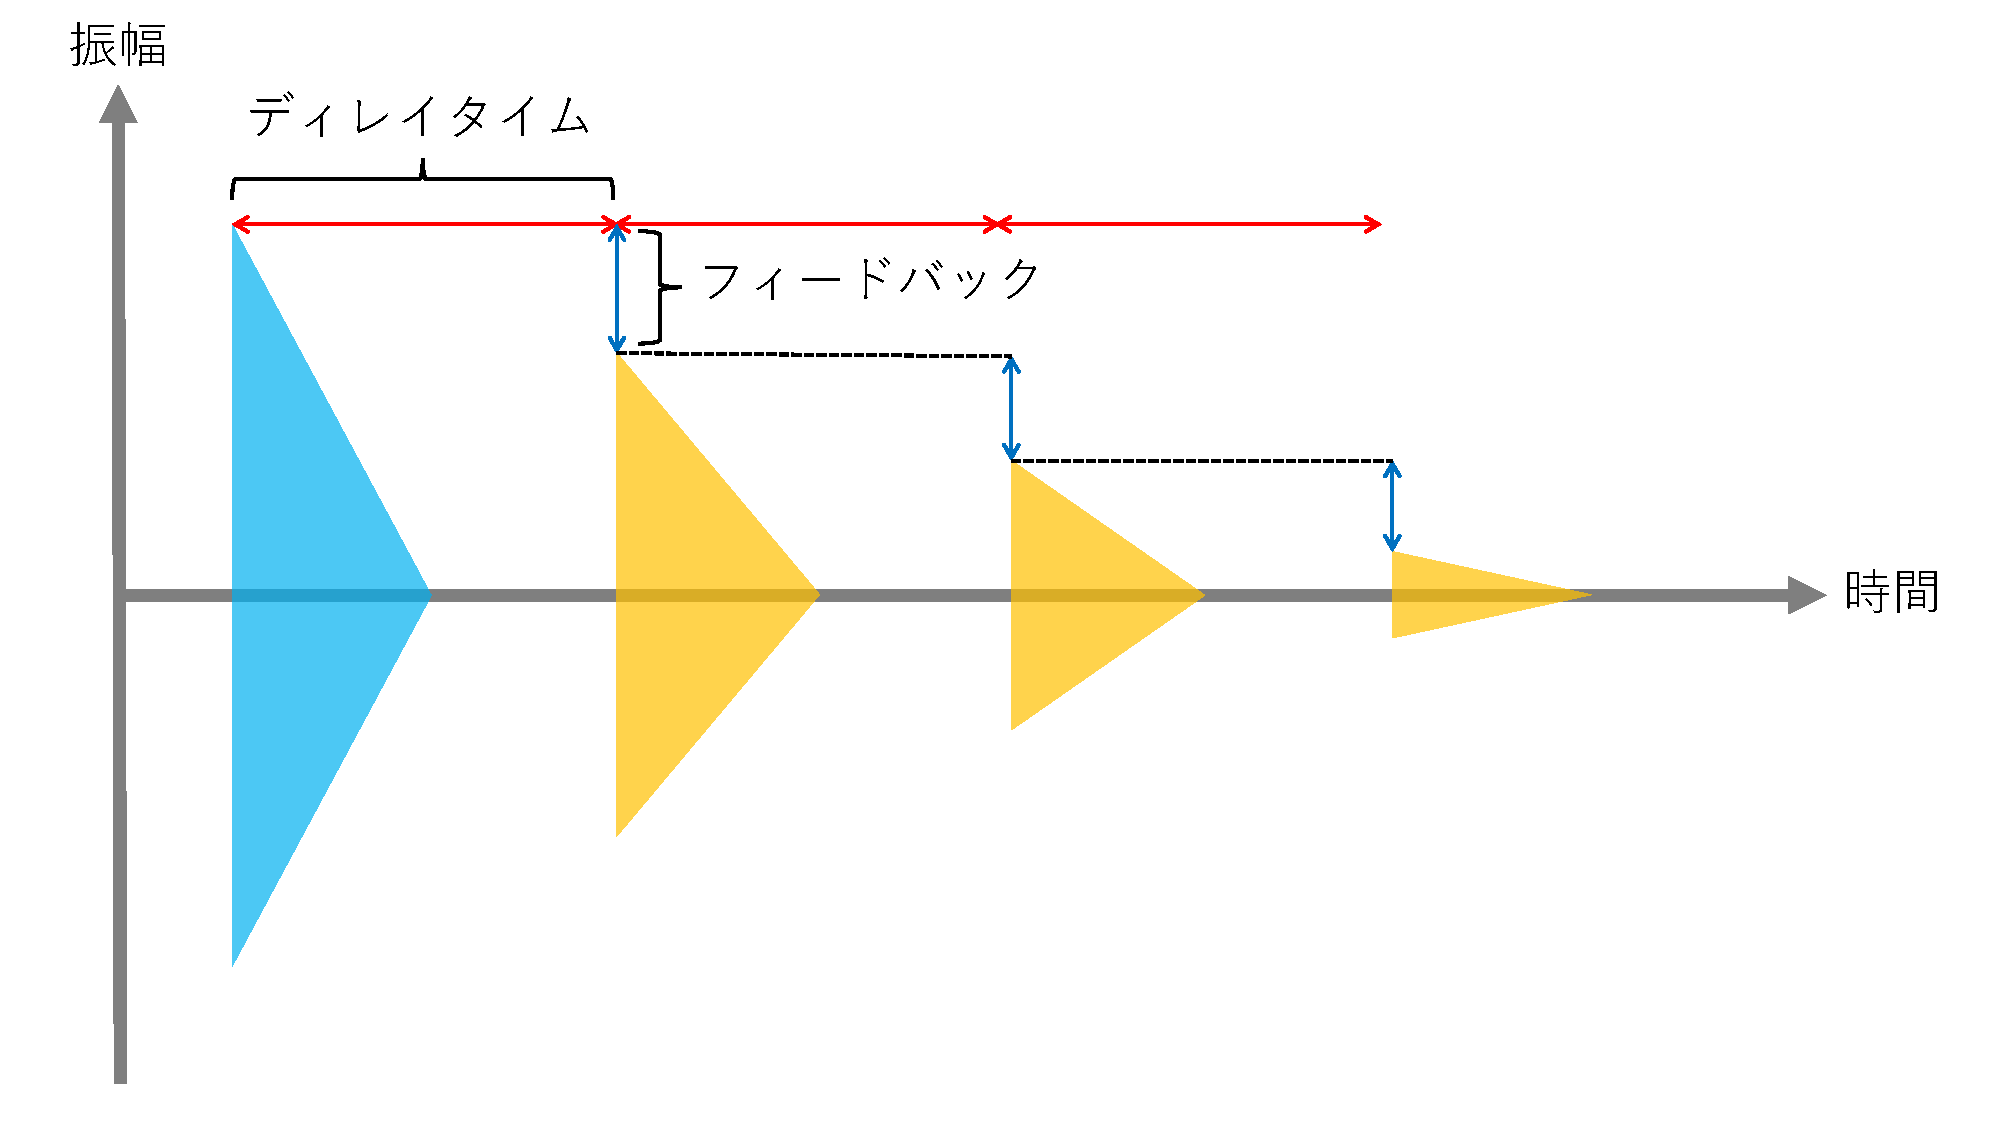
\includegraphics[width=120mm]{./figures/delay.pdf}
 \caption{ディレイのイメージ図}
 \label{fig:delay}
\end{figure}


\subsection{リバーブ}
リバーブは,反響音を追加するエフェクターである.
ミックスダウンにおいてのリバーブは,楽器の奥行を演出するために使われる.

リバーブのパラメーターには主にディケイ,プレディレイ,ミックス,サイズなどがある.

ディケイは,どの程度リバーブの反響音を残すかの時間である.

プレディレイは,原音がなってからどの程度,反響音を鳴らすかを遅らせる時間である.

ミックスは,原音と反響音をどの程度の比率で鳴らすかの割合である.
これを原音をドライ,反響音をウェットとして別々に設定するものもある.

サイズは,どのくらいの部屋の広さを再現するかを設定する値である.
スタジオやホールなど,それぞれの部屋の広さを個別に指定する場合もある.

どのパラメーターも,曲のジャンルや曲の中の展開でも設定の仕方は変わってくる.
例えば,ボーカルの雰囲気に合わせて深くリバーブを与える場合や,近くにある印象を持たせるために浅く与える場合もある.


\newpage
\section{開発するシミュレータ教材について}
\subsection{学習の流れ}
学習の流れを図\ref{fig:flow}に示す.
学習者は,まず別ページでエフェクターの効果と変化を文字を読んで確認する.
次に,シミュレータのページに行き,あらかじめ用意された音源とパラメーターのプリセットでエフェクターの効果のオン・オフを切り替えてその変化を聞いて確認する.
その後,ユーザーの持っている音源を読み込み,ユーザー自身がパラメーターを調整して,より理解を深めていくという流れを想定している.

\begin{figure}[H]
\centering
 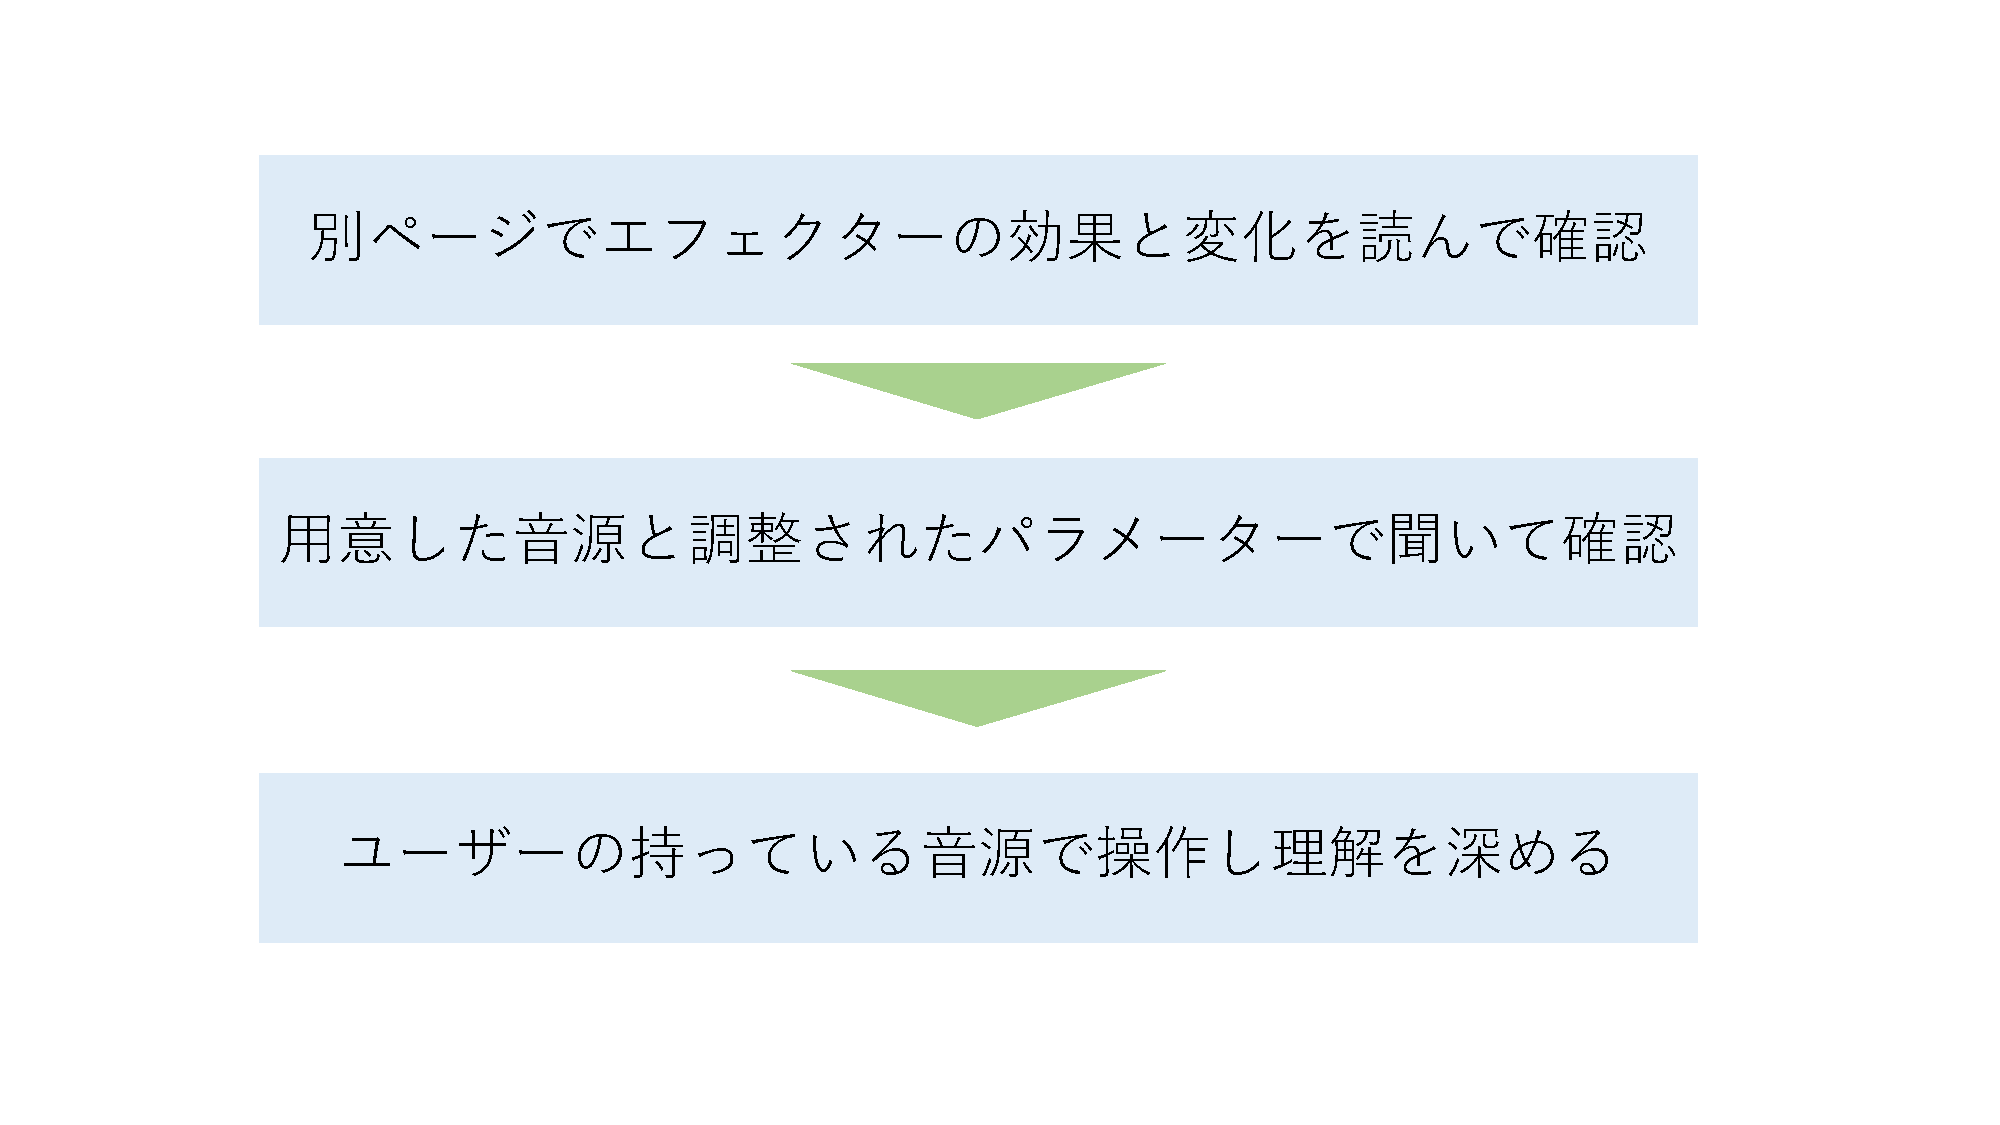
\includegraphics[width=120mm]{./figures/flow.pdf}
 \caption{学習の流れ}
 \label{fig:flow}
\end{figure}

\subsection{画面構成}
シミュレータのレイアウトを図\ref{fig:layout}に示す.
\raise0.2ex\hbox{\textcircled{\scriptsize{1}}}は,音源を操作するためのコントローラーであり,それを縦に6つ並べている.
ボタンは左から,ファイルの読み込み,ミュート,単体再生,エフェクターの効果のオン・オフ,リセット,効果を与える音源の切り替えである.赤丸は選択中の音源を表す.

「ファイルを選択」を押すことでファイルの読み込みは,mp3,oggのファイルが読み込むことができる.

「Mute」を押すことでその音源をミュートにすることができ,押すとボタンが赤くなる.
ミュートをすると,そのトラックの音源のボリュームの操作ができなくなる.

「Solo」を押すことでその音源を単体で再生することができ,押すとボタンが赤くなる.
単体再生をすると,そのトラック以外の「Mute」と「Solo」のボタンが操作できなくなる.

「Bypass」を押すことでその音源のエフェクターの効果をオフにすることができる.
オフの時にはボタンが赤,オンの時には白になる.
オフの時には,そのトラックのエフェクターのパラメーターの操作ができなくなる.

「リセット」を押すことでその音源のすべてのパラメーターをデフォルトの値に戻し,読み込まれたファイルをそのトラックから消すことができる.

「切り替え」を押すことで押された音源のトラックを選択し,そのトラックのコントローラーに赤丸を表示し,\raise0.2ex\hbox{\textcircled{\scriptsize{3}}},\raise0.2ex\hbox{\textcircled{\scriptsize{4}}}にそのトラックのものを表示する.

\textcircled{\scriptsize{3}}に,現在選択されている音源のファイル名と,エフェクターの効果のパラメーターを調整するスライダーを表示している.
ボリュームとパンのスライダーは4つのエフェクターに共通して設置している.
ボリュームとパンの下に各エフェクターのパラメーターを調整するスライダーを設置している.

\textcircled{\scriptsize{4}}に,音声波形やエフェクターの効果を表す図などを表示している.
これはイコライザーとコンプレッサーのみについている.

\begin{figure}[H]
\centering
 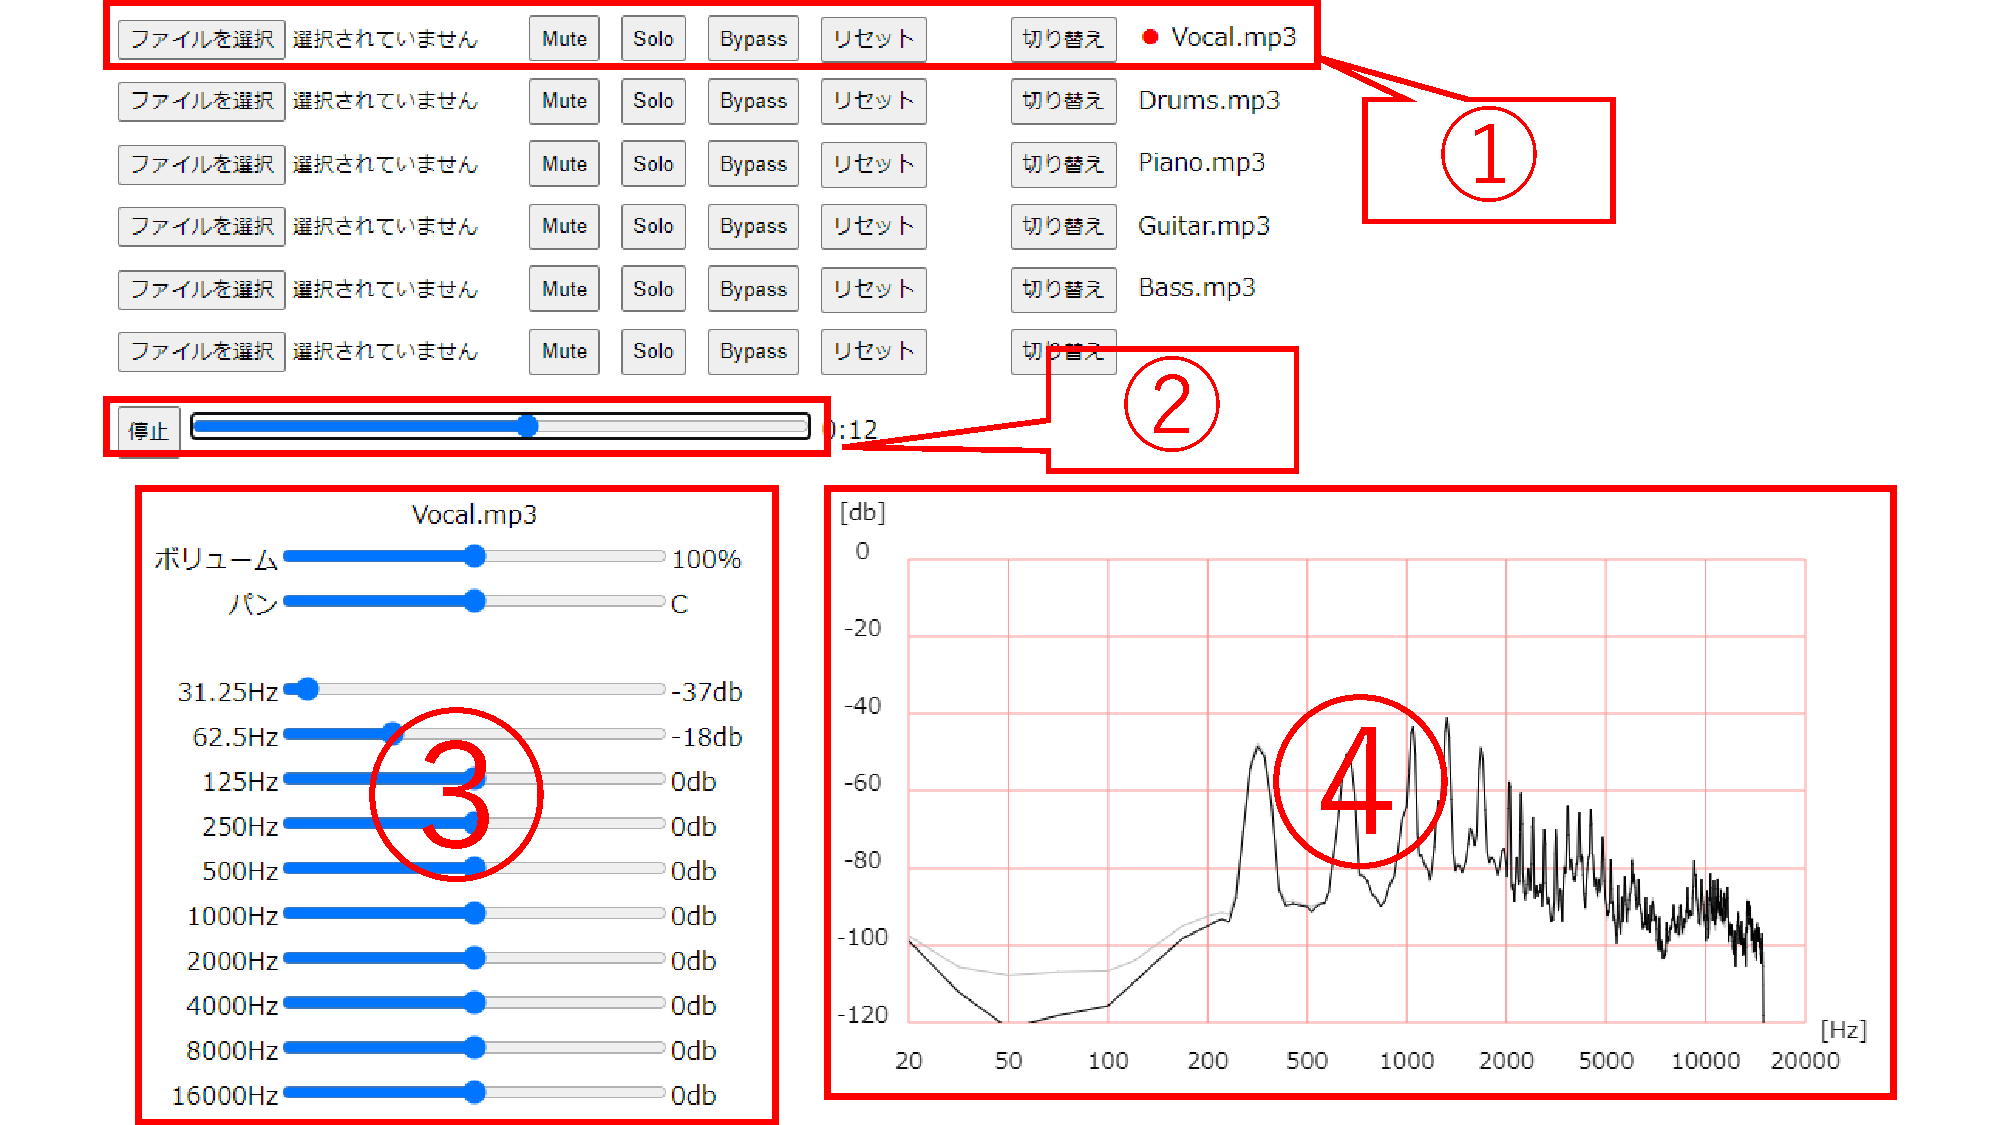
\includegraphics[width=150mm]{./figures/layout.pdf}
 \caption{シミュレータのレイアウト}
 \label{fig:layout}
\end{figure}

\subsection{パラメーターと図}
この節では,各エフェクターの図\ref{fig:layout}の\raise0.2ex\hbox{\textcircled{\scriptsize{3}}}にどのようなパラメーターがあるのか,\raise0.2ex\hbox{\textcircled{\scriptsize{4}}}にどのような図が表示されるのかを説明する.
\subsubsection{イコライザー}
イコライザーのパラメーターと表示を図\ref{fig:EQlayout}に示す.
イコライザーのパラメーターには10個あり,31.25\sim16000Hzまでを段階的に調整できる.
各周波数,-40\sim40dbまで1刻みで調整できる.

イコライザーの図は,縦軸が音量,横軸が周波数のグラフがリアルタイムで描画される.
またグラフの黒い線がイコライザーを通した音の波形で,灰色の線がイコライザーを通す前の音を表し,どこの周波数帯をどのくらい操作したのかを視覚的に理解できるようになっている.

\begin{figure}[H]
\centering
 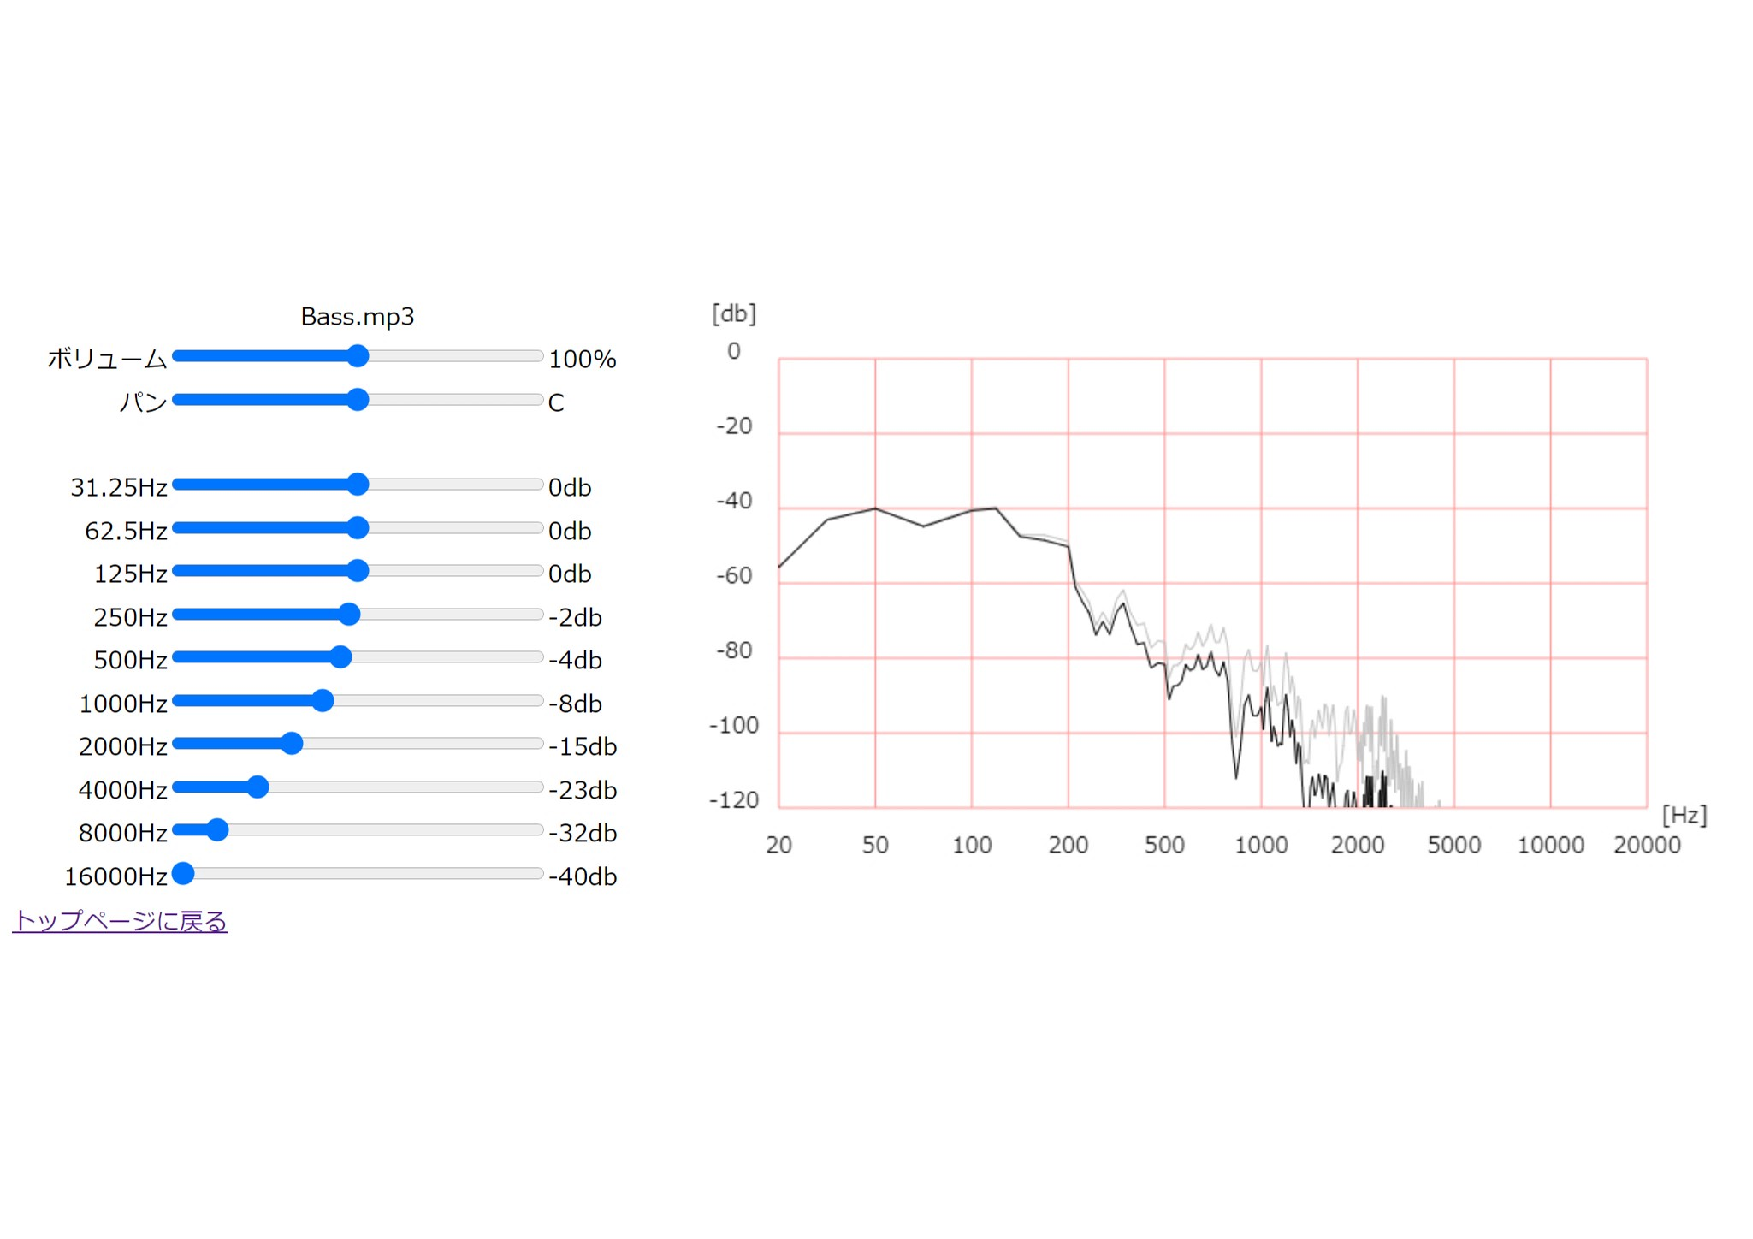
\includegraphics[width=150mm]{./figures/EQlayout.pdf}
 \caption{イコライザーのパラメーターと表示}
 \label{fig:EQlayout}
\end{figure}

\subsubsection{コンプレッサー}
コンプレッサーのパラメーターと表示を図\ref{fig:Complayout}に示す.
コンプレッサーのパラメーターには4つあり,スレショルド,レシオ,アタック,リリースがある.
スレショルドは-80\sim0dbまで1刻み,レシオは1\sim20まで0.1刻み,アタックは0\sim1秒まで0.001刻み,リリースは0.001\sim1秒まで0.001刻みで調整できる.

コンプレッサーの図は2つある.
左にある図は縦軸が出力音量,横軸が入力音量となっている.
オレンジ色の線がスレショルド,スレショルドより上の線の曲がり具合がレシオを表し,どのくらいの音量がどのくらい圧縮されるのかが視覚的に理解できるようになっている.

右にある図は縦軸が音量となっている.
青い線がコンプレッサーを通した後の音量,赤い線がコンプレッサーを通す前の音量を表し,現在出ている音がどのくらいの音量なのかが視覚的に理解できるようになっている.

\begin{figure}[H]
\centering
 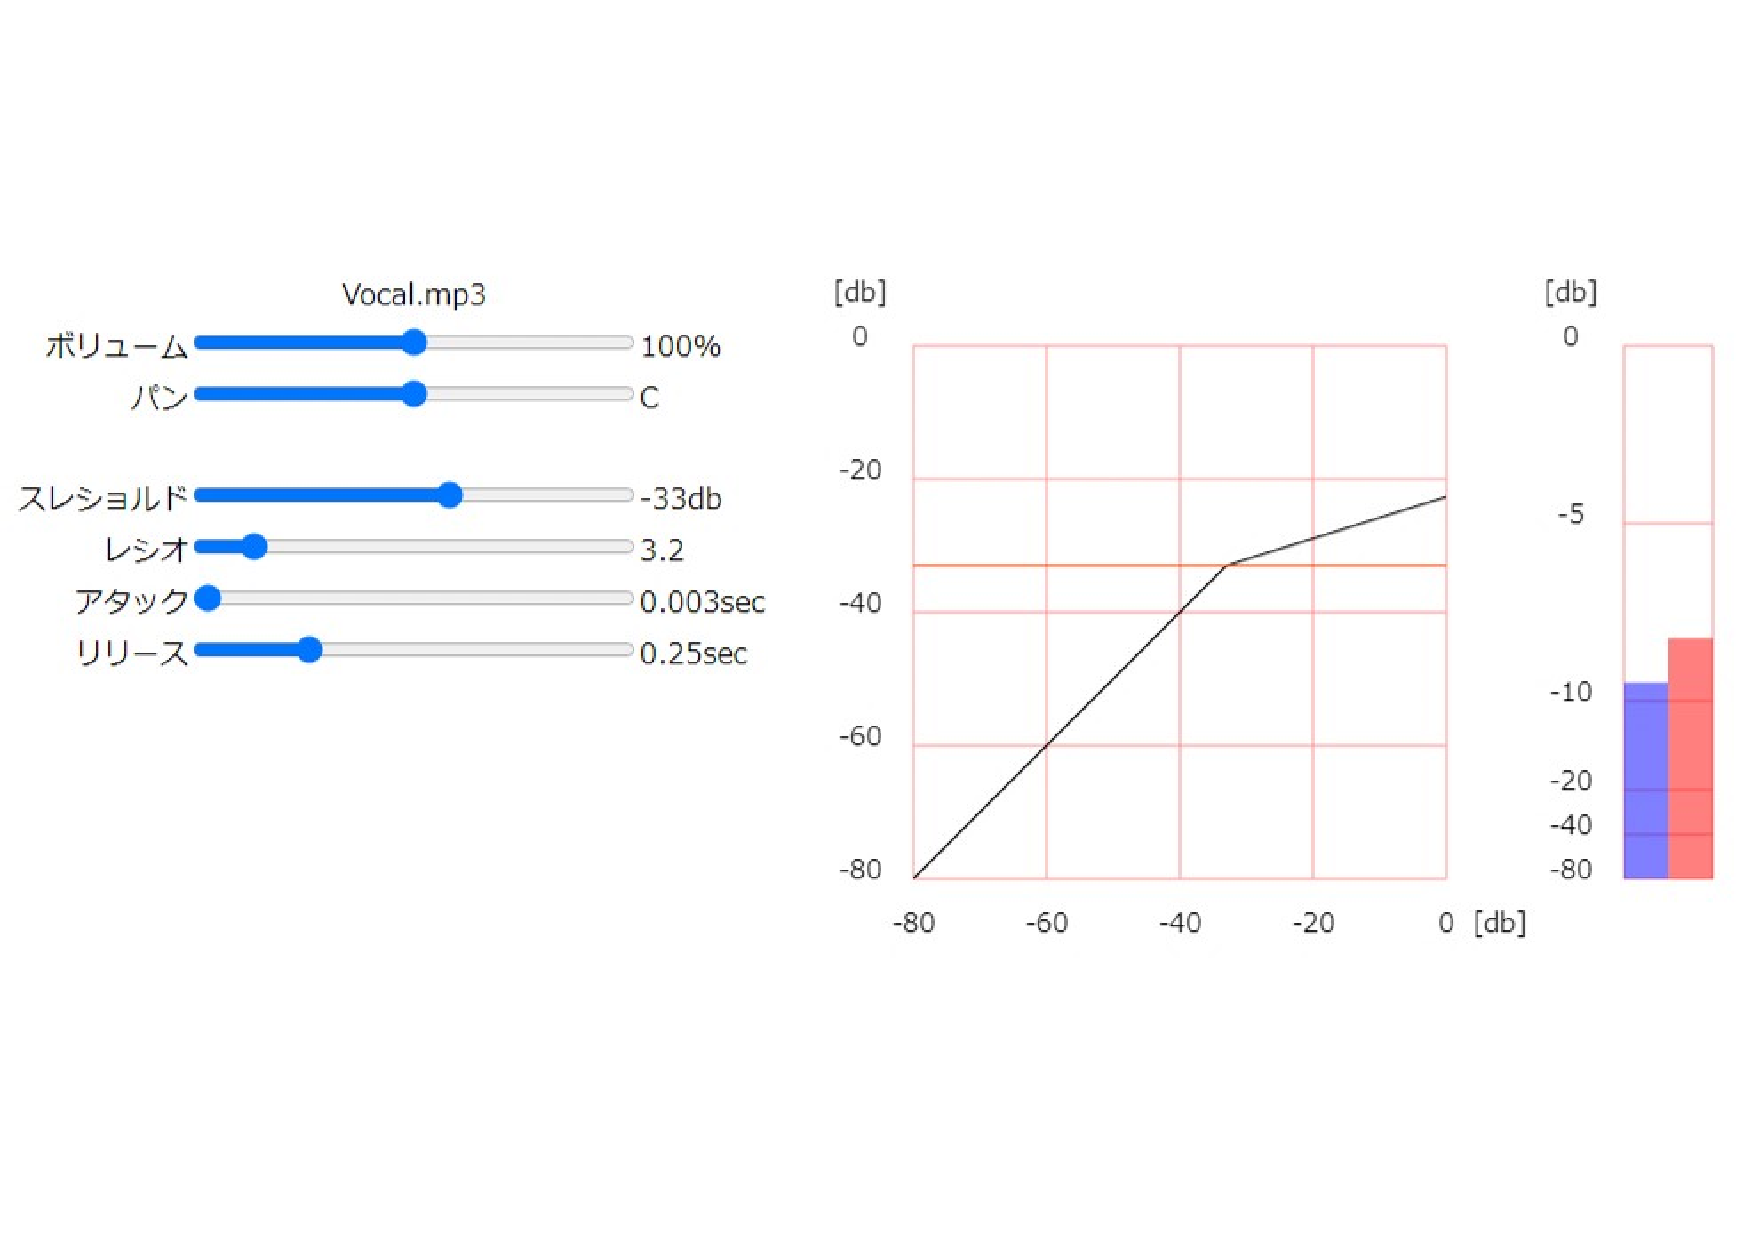
\includegraphics[width=150mm]{./figures/Complayout.pdf}
 \caption{コンプレッサーのパラメーターと表示}
 \label{fig:Complayout}
\end{figure}

\subsubsection{ディレイ}
ディレイのパラメーターを図\ref{fig:delaylayout}に示す.
ディレイのパラメーターには2つあり,ディレイタイム,フィードバックがある.
ディレイタイムは0\sim1秒まで0.01刻み,フィードバックは0\sim0.9まで0.1刻みで調整できる.

\begin{figure}[H]
\centering
 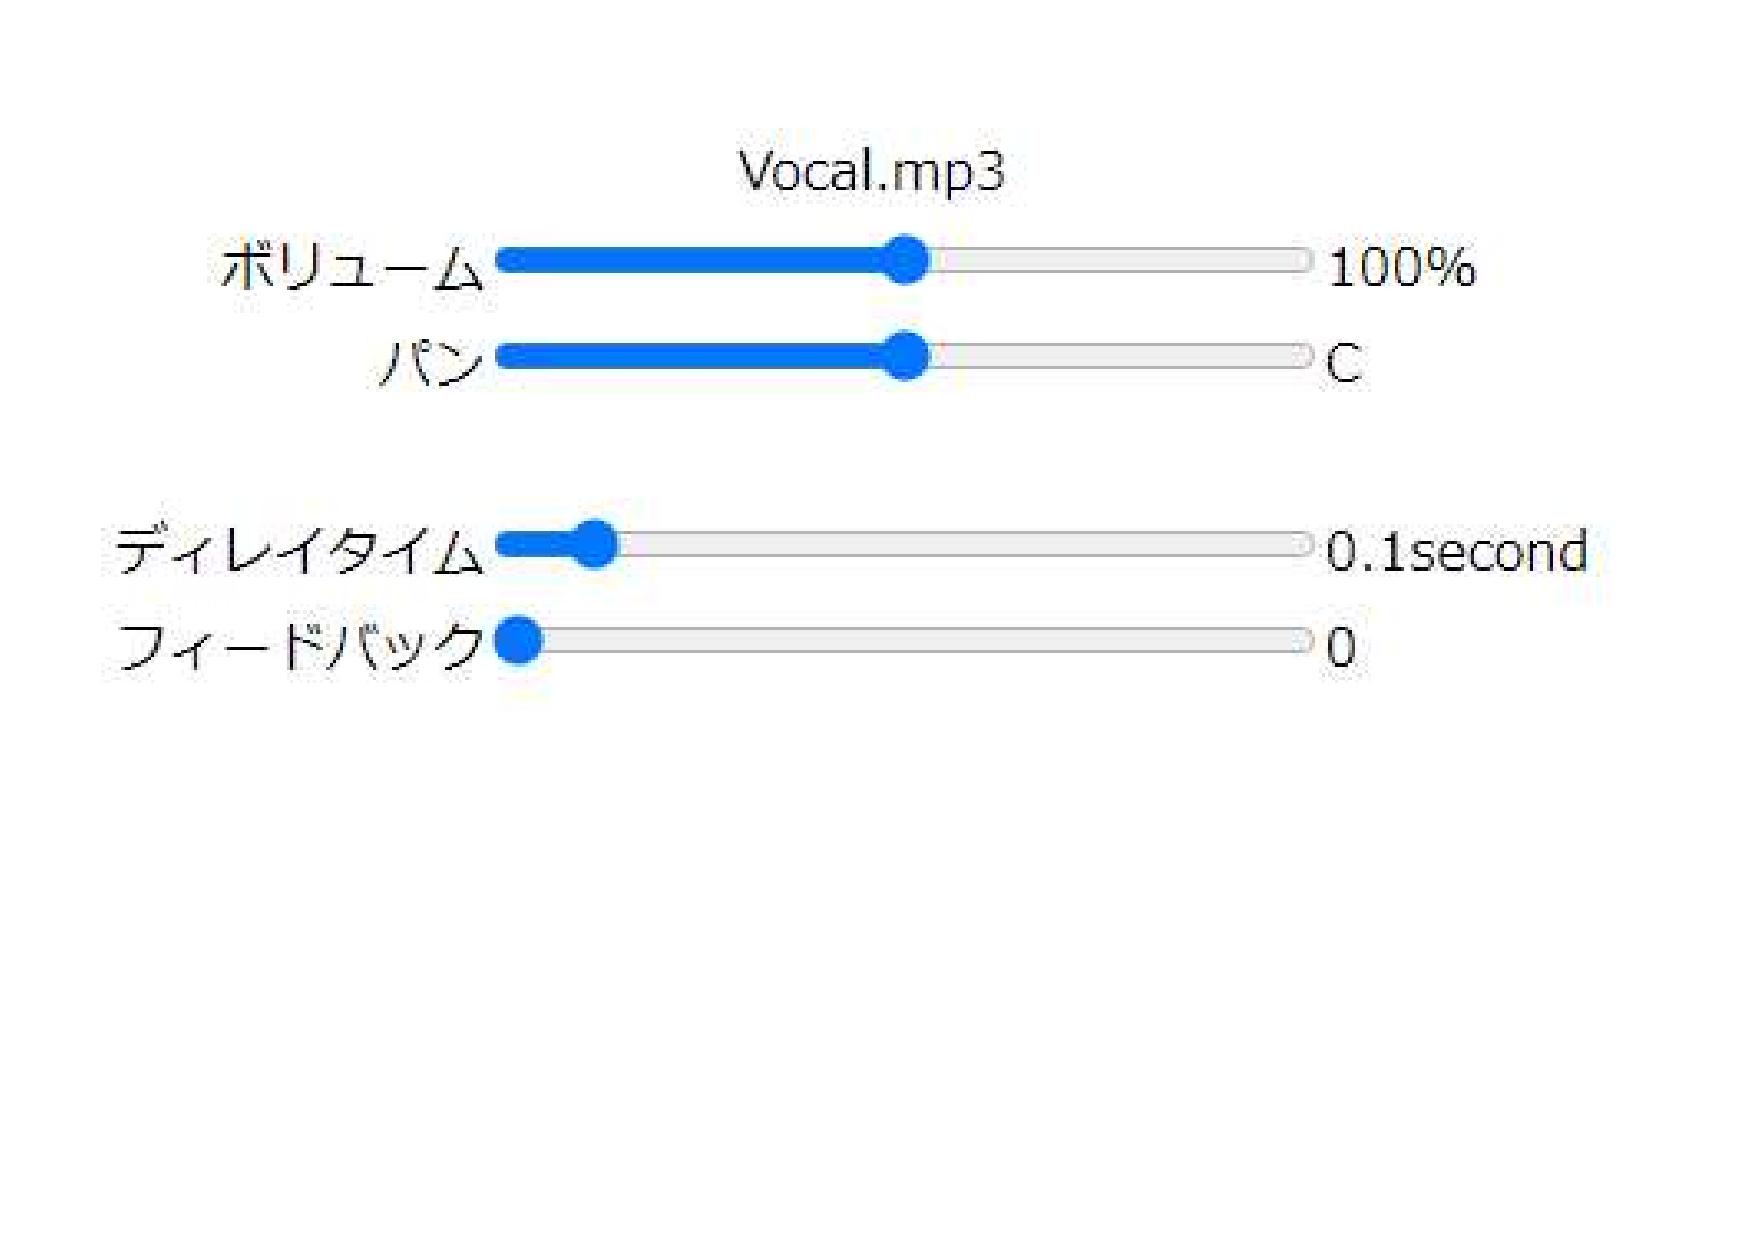
\includegraphics[width=100mm]{./figures/delaylayout.pdf}
 \caption{ディレイのパラメーター}
 \label{fig:delaylayout}
\end{figure}

\subsubsection{リバーブ}
リバーブのパラメーターを図\ref{fig:reverblayout}に示す.
リバーブのパラメーターには2つあり,ウェット,ドライがある.
ウェット,ドライはともに0\sim1まで0.1刻みで調整できる.

\begin{figure}[H]
\centering
 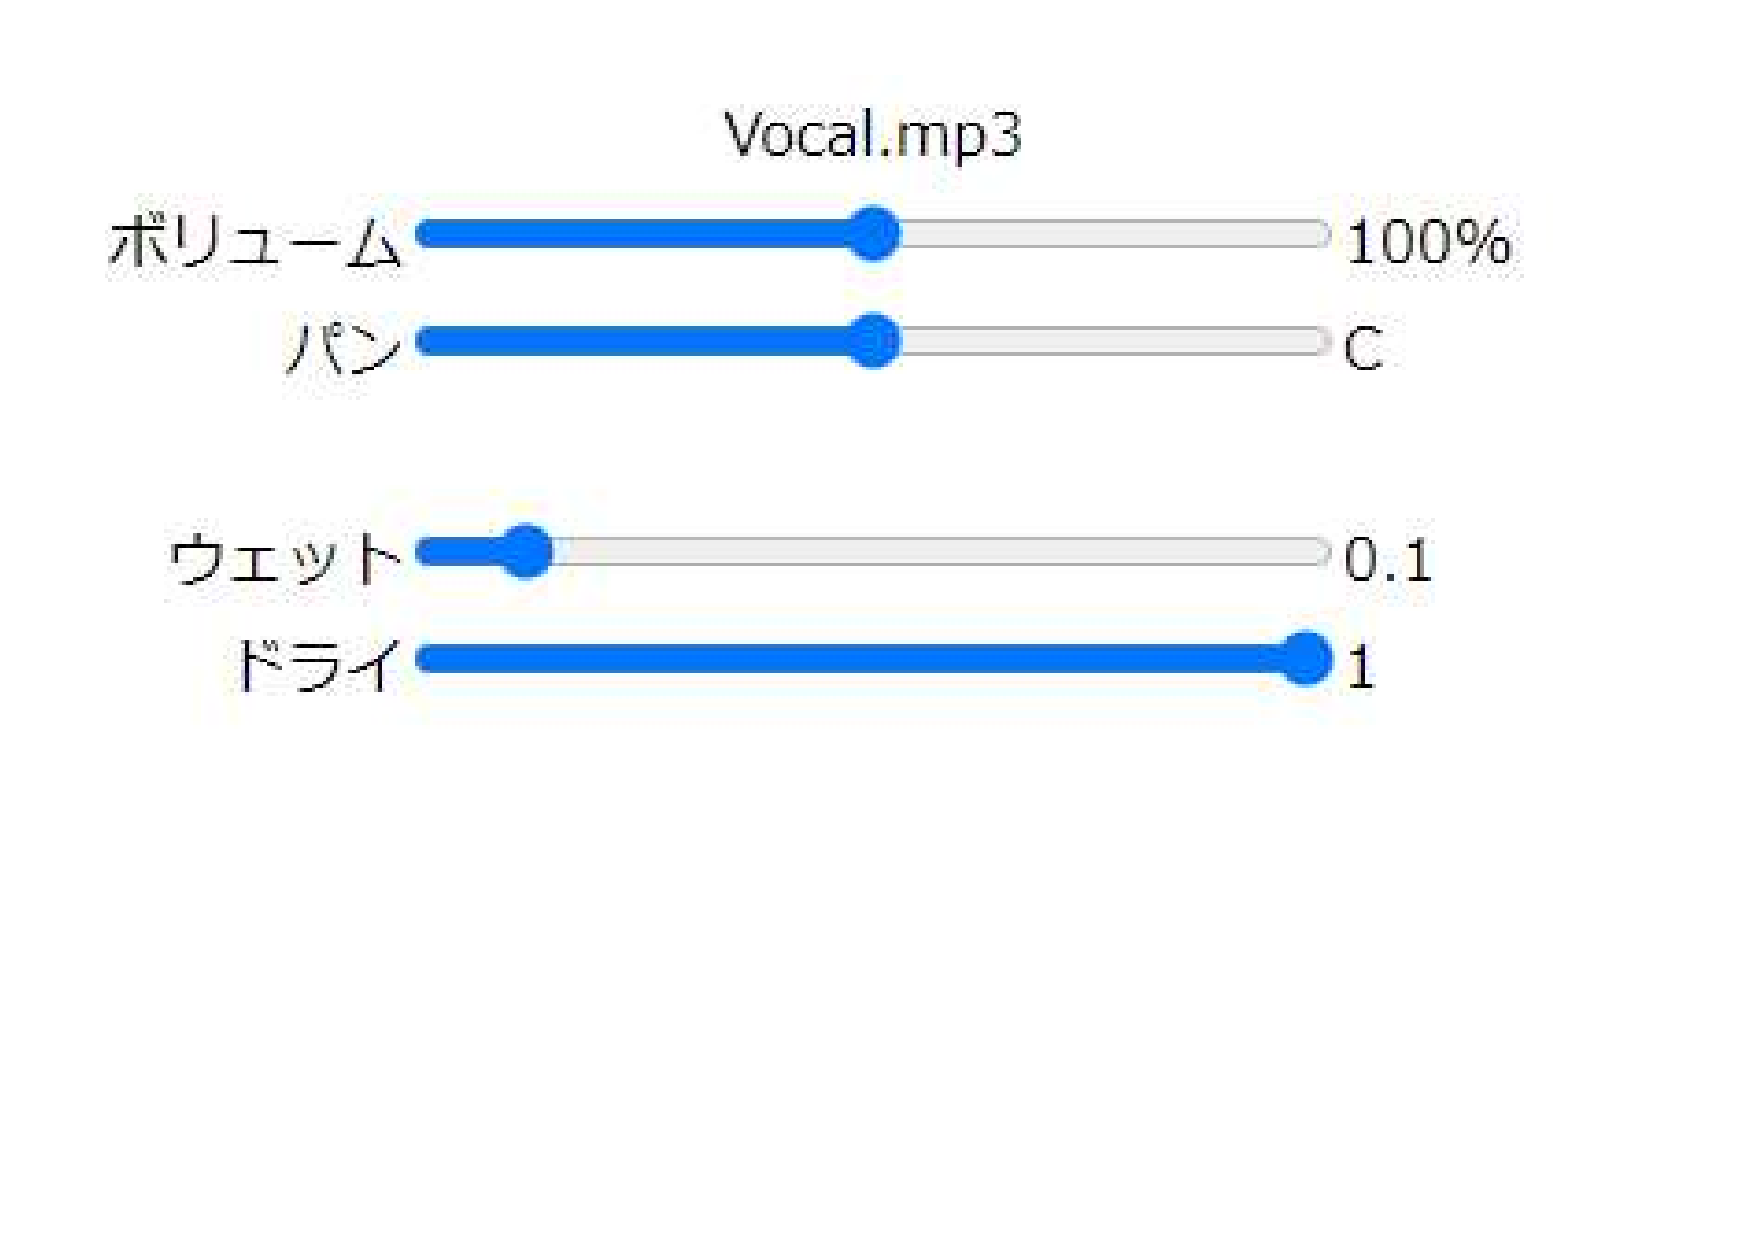
\includegraphics[width=100mm]{./figures/reverblayout.pdf}
 \caption{リバーブのパラメーター}
 \label{fig:reverblayout}
\end{figure}

\newpage
\section{制作に使用した技術}
この章では制作で使用した技術について解説する.
\subsection{HTML}
HTMLとは「HyperText Markup Language」の略称であり,Webページのテキストや構造を定義するためのマークアップ言語である\cite{html}.
ブラウザでは,HTMLファイルに書かれた通りの動かない静的なページが表示される.

\subsubsection{HTML5}
HTML5は,HTMLの5つめのバージョンのことである.
2014年にHTML5が発表され,現在の主流のバージョンとなっている.
HTML5は,ページに動画や音声の埋め込むことが簡単になったことや,文章構造が以前よりもシンプルになったという特徴がある\cite{html5}.
以前はプラグインを使用して,音声や動画,図形の描画などをしていたが,HTML5では,音声はaudioタグ,動画はvideoタグ,図形の描画はcanvasタグで簡単にできるようになった.

\subsubsection{HTMLの書き方}
HTMLの書き方は,役割をもったタグというものを使い書いていく.
HTMLは,headタグ,bodyタグで構成される.

headタグの内容は,ウェブページの情報を表し,実際にブラウザ上では表示されない.
headタグの中には,タイトル,言語情報,文字コード,JavaScript,CSSのファイルの場所などの情報を書く.

bodyタグは実際に画面に表示する内容を書く.
bodyタグの中には,通常のテキスト以外にも,hタグで見出しのテキスト,fontタグでフォントや大きさ,色を指定して書くことができる.
また文字だけではなく,ボタンやテキストボックスを表示させるinputタグ,画像を表示させるimgタグ,音声を流すaudioタグ,動画を再生させるvideoタグなど様々なものがある.

\newpage
\subsection{JavaScript}
JavaScriptは,Webページを動かすためのプログラミング言語である.
HTMLでは動かない静的なページしか作れないが,JavaScriptを用いることにより動きのある動的なページを作ることができる.
例えば,HTMLのinputタグで配置したボタンがあるとする.
HTMLのみでは,ボタンを押しても画面が変わることはない.
しかしJavaScriptを使うことで,ボタンが押されたときにどのような処理をするのか,またどのようなものを表示させるかなどを登録して,その動作を実際にブラウザ上に表示させ,動きを作ることができる.

\subsubsection{Javaとの関係}
プログラミング言語のひとつにJavaというものがある.
JavaとJavaScriptは名前が似ているだけで,全く別のプログラミング言語である.
JavaScriptは開発された時は「LiveScript」という名前だったが,当時に人気であったJavaにあやかり「JavaScript」という名前に変更された.

\subsubsection{JavaScriptの書き方}
JavaScriptを記述する方法は,HTMLのscriptタグ内に直接書き込むか,外部のファイルに書いて,それをHTMLで指定するかの2種類がある.
JavasScriptでは,変数,if文やfor文などの制御構造,関数,クラスなどを使ってプログラムを書く.

変数はデータを格納するもので数値や文字列や配列を保存することができる.
変数の宣言には,「var」「let」「const」を使う.
varとletは,代入した値を後から変更できる変数であり,constは,一度代入した値を変更できない変数である.
varは宣言した変数をもう一度宣言することができる変数であり,letは宣言した変数は再度宣言できない変数である.

制御構造はプログラムの基本的な処理のことをいい,if,for,whileなどがある.
ifは分岐を表し,条件によって処理を変えることができる.
forとwhileは繰り返しを表し,forは回数を指定して繰り返し,whileは指定した条件になっている間に繰り返す.

関数は,処理を1つにまとめたものをいう.
関数を使用するには,関数を定義する必要がある.
関数の名前を指定し,その関数が行う処理を記述することで,関数を定義することができる.
定義したあとは,その関数の名前を書くことで,その処理を実行することができる.

クラスは,変数や関数をまとめた設計図みたいなものである.
クラスを使用するには,クラスを定義する必要がある.
クラスには,変数,関数,インスタンス化したときに処理をする特殊な関数のコンストラクターを記述することで,クラスを定義することができる.
クラスを使うには,インスタンス化する必要がある.
インスタンス化とは,オブジェクトという変数のようなものにクラスを代入することである.
インスタンス化することで,クラスはインスタンスになる.
それぞれのインスタンスには,クラスで定義した関数や変数をそれぞれ持つことができ,インスタンスごとに処理をすることができる.

\subsection{Web Audio API}
Web Audio APIはWeb上で音声を様々な操作することができるAPIである.このAPIを使用すると,Webページ上で音声を合成することや,エフェクターの効果を与えるなどができる.

\subsubsection{API}
APIとはApplication Programming Interfaceの略称であり,外部から関数やメソッドを呼び出して,使えるようにできる仕組みのことである\cite{api}.
例えば,この制作でやりたい音声にエフェクターの効果を与えるということをする.
それを実現するプログラムを自分で書こうとすると膨大な手間がかかる.
それを外部からWeb Audio APIを呼び出すことで,関数を書くだけで簡単に実装することができる.

\subsubsection{実装方法}
音を出す手順として次のようになる.
まず生成した音源やファイルから取得した音源を出す入力点を生成する.
音を出力する出力点を生成し入力点と出力点を接続する.
最後に音源のスイッチをオンにする.
このようにすると音を出すことができる.
エフェクターの効果を与えるには,入力点と出力点の間にエフェクターを挟むことでそのエフェクターを通した音を出力することができる.

\subsubsection{制作に使用したクラス}
ここでは制作に使用したWeb Audio APIのエフェクターと可視化する図を実装するクラスとそのプロパティを書く.
使用したクラスは,ボリュームを実装するGainNode,パンを実装するStereoPannerNode,イコライザーを実装するBiquadFilterNode,コンプレッサーを実装するDynamicsCompressorNode,ディレイを実装するDelayNode,リバーブを実装するConvolverNode,可視化する図(アナライザー)を実装するAnalyserNodeである.

ボリュームを実装するGainNodeについて説明する.
GainNodeのインスタンスを生成するには,createGainメソッドを使う.
GainNodeのプロパティには1つあり,gainがある.
gainの値を操作することにより,ボリュームの大きさを変えることができる.この値はデフォルトで1,最小値が0,最大値が1と定義されている.

パンを実装するStereoPannerNodeについて説明する.
StereoPannerNodeのインスタンスを生成するには,createStereoPannerメソッドを使う.
PannerNodeのプロパティには1つあり,panがある.
panの値を操作することにより,パンの位置を変えることができる.この値はデフォルトで0,最小値が-1,最大値が1と定義されている.
マイナスにすると左側に,プラスにすると右側に定位が寄る.

イコライザーを実装するBiquadFilterNodeについて説明する.
BiquadFilterNodeのインスタンスを生成するには,createBiquadFilterメソッドを使う.
BiquadFilterNodeのプロパティには4つあり,frequency,Q,detune,gainがある.
BiquadFilterNodeのプロパティを表\ref{table:biquadfilternode}に示す.
frequencyは,調整するイコライザーの中心の周波数を表す.この値はデフォルトで350,最小値は0,最大値がサンプリング周波数の1/2と定義されている.
Qは,frequencyからの幅の広さを表す値である.この値はデフォルトで0,最小値が-∞,最大値が+∞と定義されている.
detuneは,frequencyからの周波数のずれを表す値である.この値はデフォルトで1,最小値が-∞,最大値が+∞と定義されている.
gainは,調整する周波数の音量の大きさを表す値である.この値はデフォルトで0,最小値が-∞,最大値が+∞と定義されている.

\begin{table}[h]
  \centering
  \caption{BiquadFilterNodeのプロパティ}
  \label{table:biquadfilternode}
  \small
  \begin{tabular}{cccc}
    \hline
    プロパティ  & 説明 & デフォルト & 範囲    \\
    \hline \hline
    frequency  & 調整するイコライザーの中心の周波数 & 350 & 0 ~ サンプリング周波数の1/2\\
    \hline
    Q  & 帯域幅 & 0 & -∞ ~ +∞\\
    \hline
    detune  &  frequencyからの周波数のずれ & 1 & -∞ ~ +∞\\
    \hline
    gain  &  調整する周波数の音量の大きさ & 0 & -∞ ~ +∞\\
    \hline
  \end{tabular}
\end{table}

コンプレッサーを実装するDynamicsCompressorNodeについて説明する.
DynamicsCompressorNodeのインスタンスを生成するには,createDynamicsCompressorメソッドを使う.
DynamicsCompressorNodeのプロパティには6つあり,threshold,knee,ratio,attack,release,reductionがある.
DynamicsCompressorNodeのプロパティを表\ref{table:DynamicsCompressorNode}に示す.
thresholdは,圧縮される音量の閾値を表す.この値はデフォルトで-24,最小値は-100,最大値が0と定義されている.
kneeは,音量が圧縮される滑らかさを表す.この値はデフォルトで30,最小値は-100,最大値が0と定義されている.
ratioは,圧縮される割合を表す.この値はデフォルトで12,最小値は1,最大値が20と定義されている.
attackは,閾値を超えてから圧縮されるまでの時間を表す.この値はデフォルトで0.003,最小値は0,最大値が1と定義されている.
releaseは,閾値を下回ってから圧縮をやめるまでの時間を表す.この値はデフォルトで0.250,最小値は0,最大値が1と定義されている.
reductionは,コンプレッサーの現在の減衰量を表す.この値は読み取り専用である.
本来,コンプレッサーは音量を圧縮するのみだが,DynamicsCompressorNodeで実装されるコンプレッサーは,圧縮に応じて全体の音量が上がるという仕様がある.

\begin{table}[h]
  \centering
  \caption{DynamicsCompressorNodeのプロパティ}
  \label{table:DynamicsCompressorNode}
  \small
  \begin{tabular}{cccc}
    \hline
    プロパティ  & 説明 & デフォルト & 範囲    \\
    \hline \hline
    threshold  & 圧縮される音量の閾値 & -24 & -100 ~ 0\\
    \hline
    knee  & 音量が圧縮される滑らかさ & 30 & 0 ~ 40\\
    \hline
    ratio  &  圧縮される割合 & 12 & 1 ~ 20\\
    \hline
    attack  &  閾値を超えてから圧縮されるまでの時間 & 0.003 & 0 ~ 1\\
    \hline
    release  &  閾値を下回ってから圧縮をやめるまでの時間 & 0.250 & 0 ~ 1\\
    \hline
    reduction  &  コンプレッサーの現在の減衰量(読み取り専用) & - & -\\
    \hline
  \end{tabular}
\end{table}

ディレイを実装するDelayNodeのインスタンスを生成するには,createDelayメソッドを使う.
DelayNodeのプロパティには1つあり,delayTimeがある.
delayTimeは,どの程度音を遅れて出すかの時間を表す.最小値は0,最大値はcreateDelayメソッドの引数に指定した値である.
DelayNodeで実装されるディレイは,ただ単に音を遅らせるというだけで,ミックスダウンに使うようなエフェクターとしてのディレイはそのまま実装できない.
そのようなディレイはGainNodeを組み合わせて作る.
イメージ図を図\ref{fig:delaynode}に示す.
まず入力点から出た音がそのまま出力点に出て音が鳴る.
DelayNodeに入った音が遅れてGainNodeに入り音量が小さくなる.
GainNodeから出力点に入った音は出力され,再びDelayNodeに入った音が遅れてGainNodeに入り音量が小さくなる.
この繰り返しによってミックスダウンに使うようなエフェクターとしてのディレイを実装することができる.
この場合GainNodeがエフェクターのフィードバックを表すことになる.

\begin{figure}[H]
\centering
 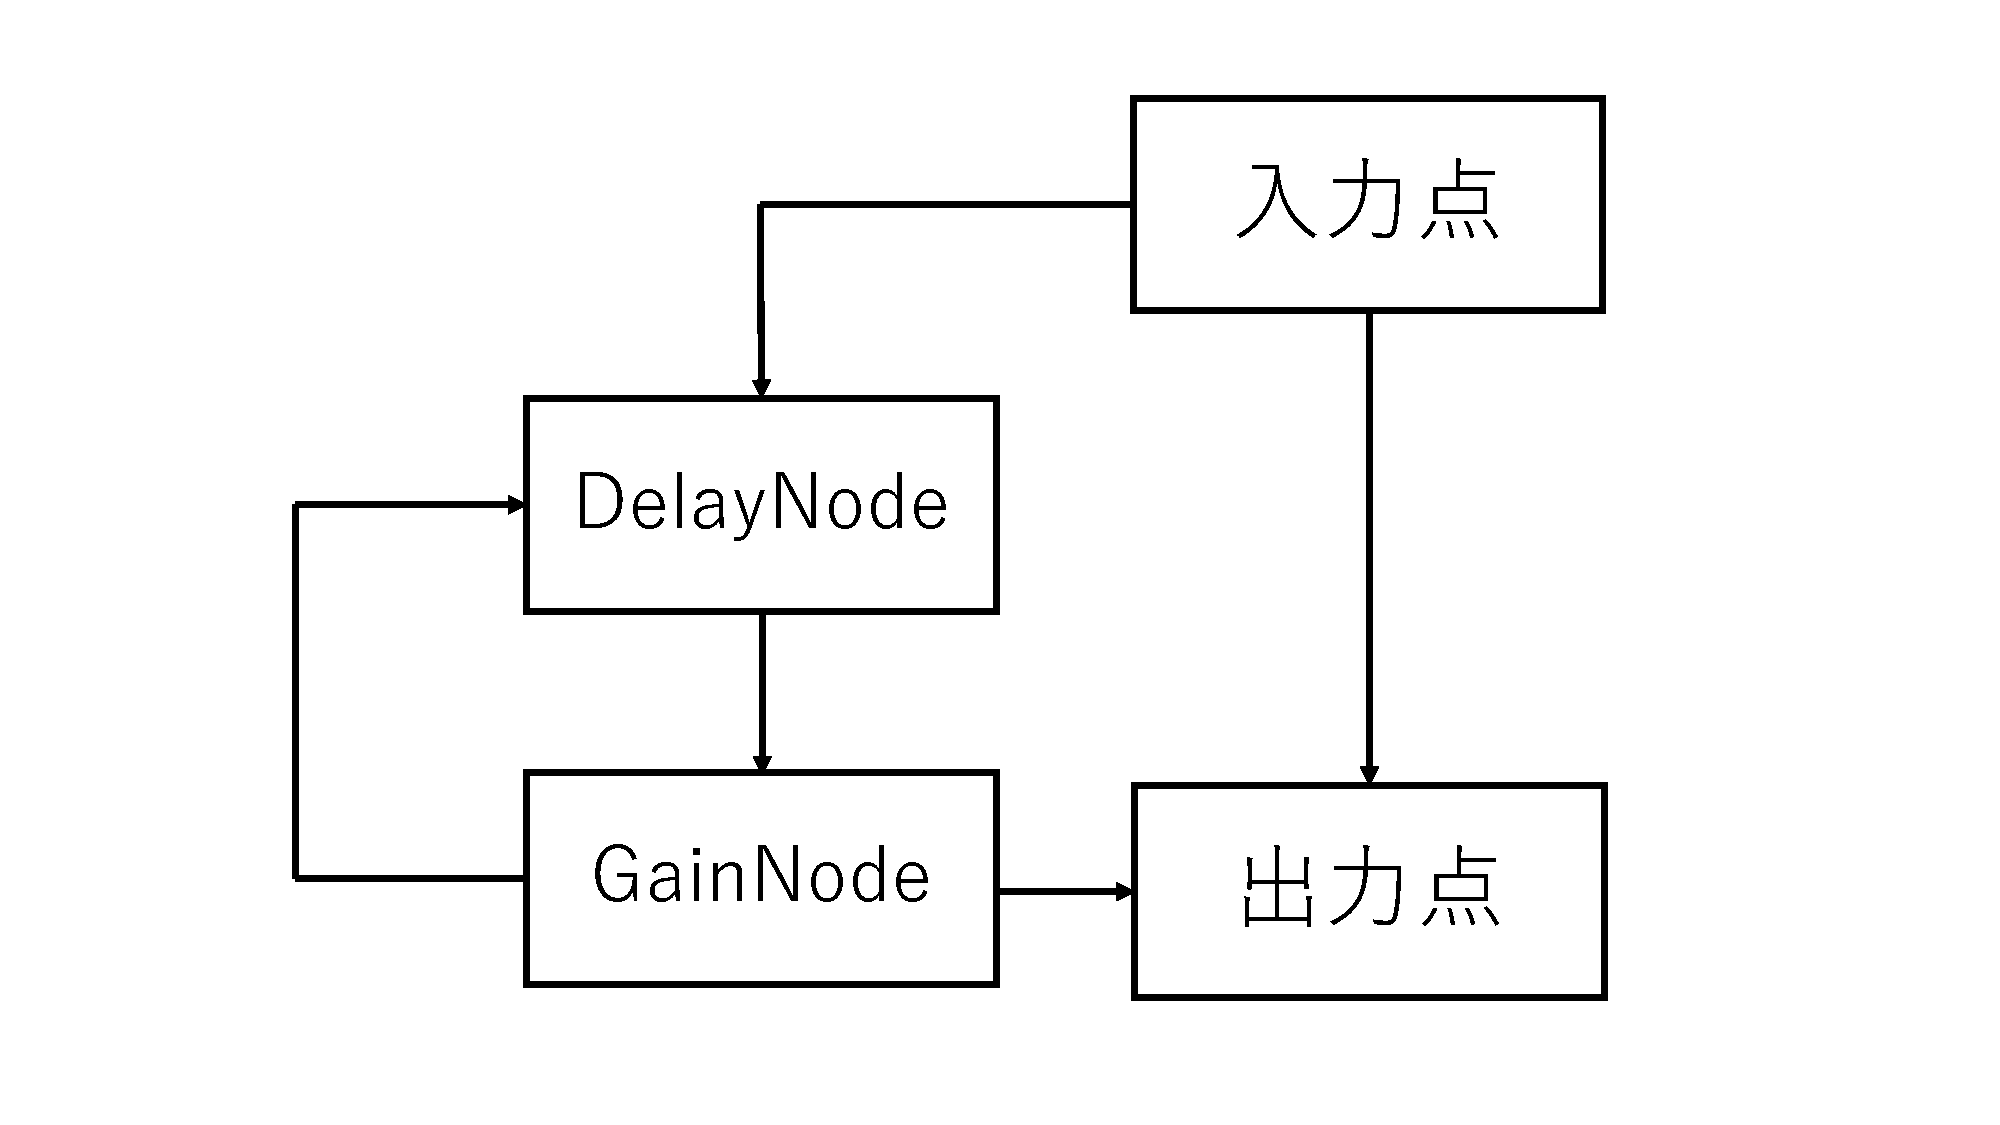
\includegraphics[width=120mm]{./figures/delaynode.pdf}
 \caption{DelayNodeとGainNode}
 \label{fig:delaynode}
\end{figure}

リバーブを実装するConvolverNodeのインスタンスを生成するには,createConvolverメソッドを使う.リバーブを実装するためにはIRデータが必要となる.
IRデータとは空間の反響を記録した短い音のデータである.
ConvolverNodeのプロパティには1つあり,bufferがある.
bufferにIRデータのバイナリデータを代入することで,そのIRデータの空間を再現したリバーブを使えるようになる.
ConvolverNodeで実装されるリバーブはそのままIRデータを適応したもので調整はできない.
そこで,音源のそのままの音(Dry)とリバーブの音(Wet)を調整できるようにGainNodeと組み合わせることでミックスダウンで使うようなエフェクターとしてのリバーブが実装できる.
イメージ図を図\ref{fig:convolvernode}に示す.
入力点から出た音を調整するためのGainNodeとConvolverNodeで処理された音を調整するためのGainNodeを用意し繋げることでリバーブの音の調整ができるようになる.

\begin{figure}[H]
\centering
 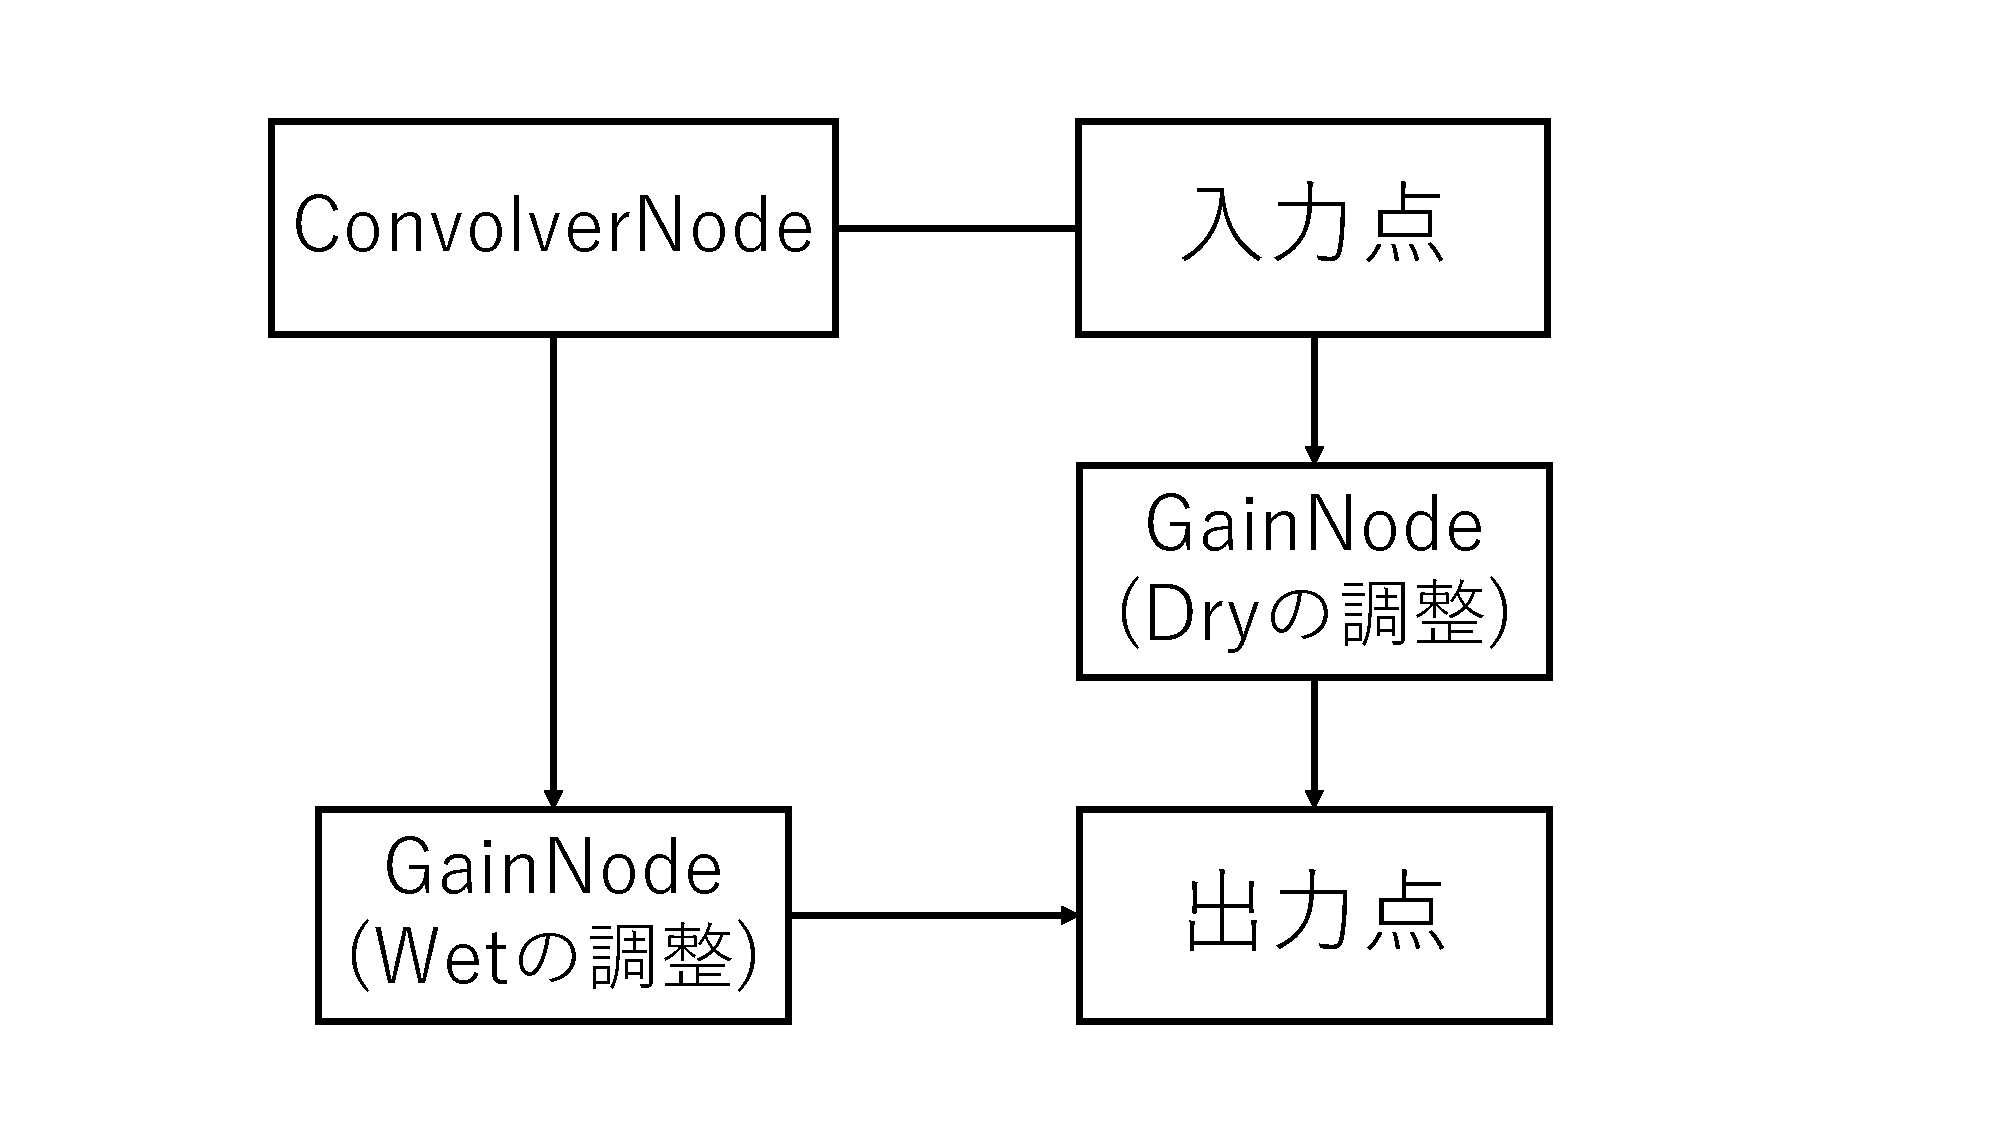
\includegraphics[width=120mm]{./figures/convolvernode.pdf}
 \caption{ConvolverNodeとGainNode}
 \label{fig:convolvernode}
\end{figure}

ディレイを実装するAnalyserNodeのインスタンスを生成するには,createAnalyserメソッドを使う.
AnalyserNodeのプロパティには5つあり,fftSize,frequencyBinCount,minDecibels,maxDecibels,smoothingTimeConstantがある.
fftSizeは,高速フーリエ変換のデータサイズを表す.この値はデフォルトで2048,最小値は32,最大値が2048と定義されている.この値は32,64,128,256,512,1024,2048のみを選べる.
frequencyBinCountは,fftSizeの1/2の値で読み取り専用である.
minDecibelsはgetByteFrequencyDataで取得できるデシベルの下限でデフォルトが-100,最小値は-100,最大値が-30と定義されている.
maxDecibelsはgetByteFrequencyDataで取得できるデシベルの上限でデフォルトが-30,最小値は-100,最大値が-30と定義されている.
smoothingTimeConstantは周波数領域の描画の更新速度で,デフォルトが0.8,最小値は0,最大値が1と定義されている.

メソッドは4つあり,getByteTimeDomainData,getByteFrequencyData,getFloatTimeDomainData,getFloatFrequencyDataがある.
getByteTimeDomainDataとgetFloatTimeDomainDataは時間領域の波形描画を取得するメソッドである.
getByteFrequencyDataとgetFloatFrequencyDataは周波数領域の波形描画を取得するメソッドである.
getByteTimeDomainDataとgetByteFrequencyDataはUint8array型の配列を引数に取り,getFloatTimeDomainDataとgetFloatFrequencyDataはFloat32Array型の配列を引数に取る.
実際に描画するにはHTMLのcanvasタグとCanvas APIを使用し,描画する.

\begin{table}[h]
  \centering
  \caption{AnalyserNodeのプロパティ}
  \label{table:AnalyserNode}
  \small
  \begin{tabular}{cccc}
    \hline
    プロパティ  & 説明 & デフォルト & 範囲    \\
    \hline \hline
    fftSize  & 高速フーリエ変換のデータサイズ & 2048 & 32 ~ 2048\\
    \hline
    frequencyBinCount  & fftSizeの1/2の値(読み取り専用) & - & -\\
    \hline
    minDecibels  & getByteFrequencyDataで取得できるデシベルの下限 & -100 & -100~-30\\
    \hline
    maxDecibels  &  getByteFrequencyDataで取得できるデシベルの上限 & -30 & -100~-30\\
    \hline
    smoothingTimeConstant  &  周波数領域の描画の更新速度 & 0.8 & 0 ~ 1\\
    \hline
  \end{tabular}
\end{table}

\subsection{CSS}
CSSとはCascading Style Sheetsの略称でありウェブページの配置や見た目を指定するための言語である\cite{css}.
CSSを使うことでHTMLのタグで置いたオブジェクトの配置を指定することや,フォント,色などを変えることができる.
\subsubsection{CSSの書き方}
CSSを記述する方法は,HTMLのstyleタグ内に直接書き込むか,外部のファイルに書いて,それをHTMLで指定するかの2種類がある.CSSでは,どこを変えるのかという対象を表す「セレクタ」,そのセレクタの持っている属性を表す「プロパティ」,プロパティをどのように変えるのかというのを表す「値」がある.

セレクタでは,HTMLで指定したIDやCLASS,範囲内のタグなどを指定する.
IDの場合は「\#」,CLASSの場合は「.」をつけて指定する.
例えば以下のようなHTMLのコードがある
\begin{lstlisting}
<div class="example_div">
  <span id="example_span2">test</span>
<div>
<div class="example_div2">
  <span>test</span>
<div>
\end{lstlisting}
ここでexample\_divを指定する場合,クラスなので「.example\_div」と書く.
example\_div内にあるspanを指定する場合は2つある.
まずIDを直接指定することで,その場合は「\#example\_span2」と書く.
もう一つはexample\_divのspanということを指定することで,その場合は「.example\_div span」と書く.
全体のspanを指定する場合は「span」と書く.
このようにするとHTML内のすべてのspanが指定される.

プロパティでは,色,フォント,高さ,幅,余白などを指定する.
ここではプロパティの例として,この制作で使用したものを説明する.
表\ref{table:css}にプロパティの例を示す.
widthは横の長さ,heightは縦の長さを表し,値はptやpxで指定する.
marginは要素の内容の外側の余白,paddingは要素の内容の内側の余白を表す.
marginのイメージ図を図\ref{fig:marginpadding}に示す.
marginの余白では背景色などは適応されないが,paddingでは適応される.
marginとpaddingの値は1つだけだと四辺すべてに適応される.
2つだと1つ目が上下,2つ目が左右に適応される.
3つだと1つ目が上,2つ目が左右,3つ目が下に適応される.
4つだと1つ目が上,2つ目が右,3つ目が下,4つ目が左に適応される.
また,プロパティでmargin-bottom,margin-left,margin-right,margin-topとpadding-bottom,margin-left,margin-right,margin-topというものがあり,それぞれ下,左,右,上を指定できる.

\begin{figure}[H]
\centering
 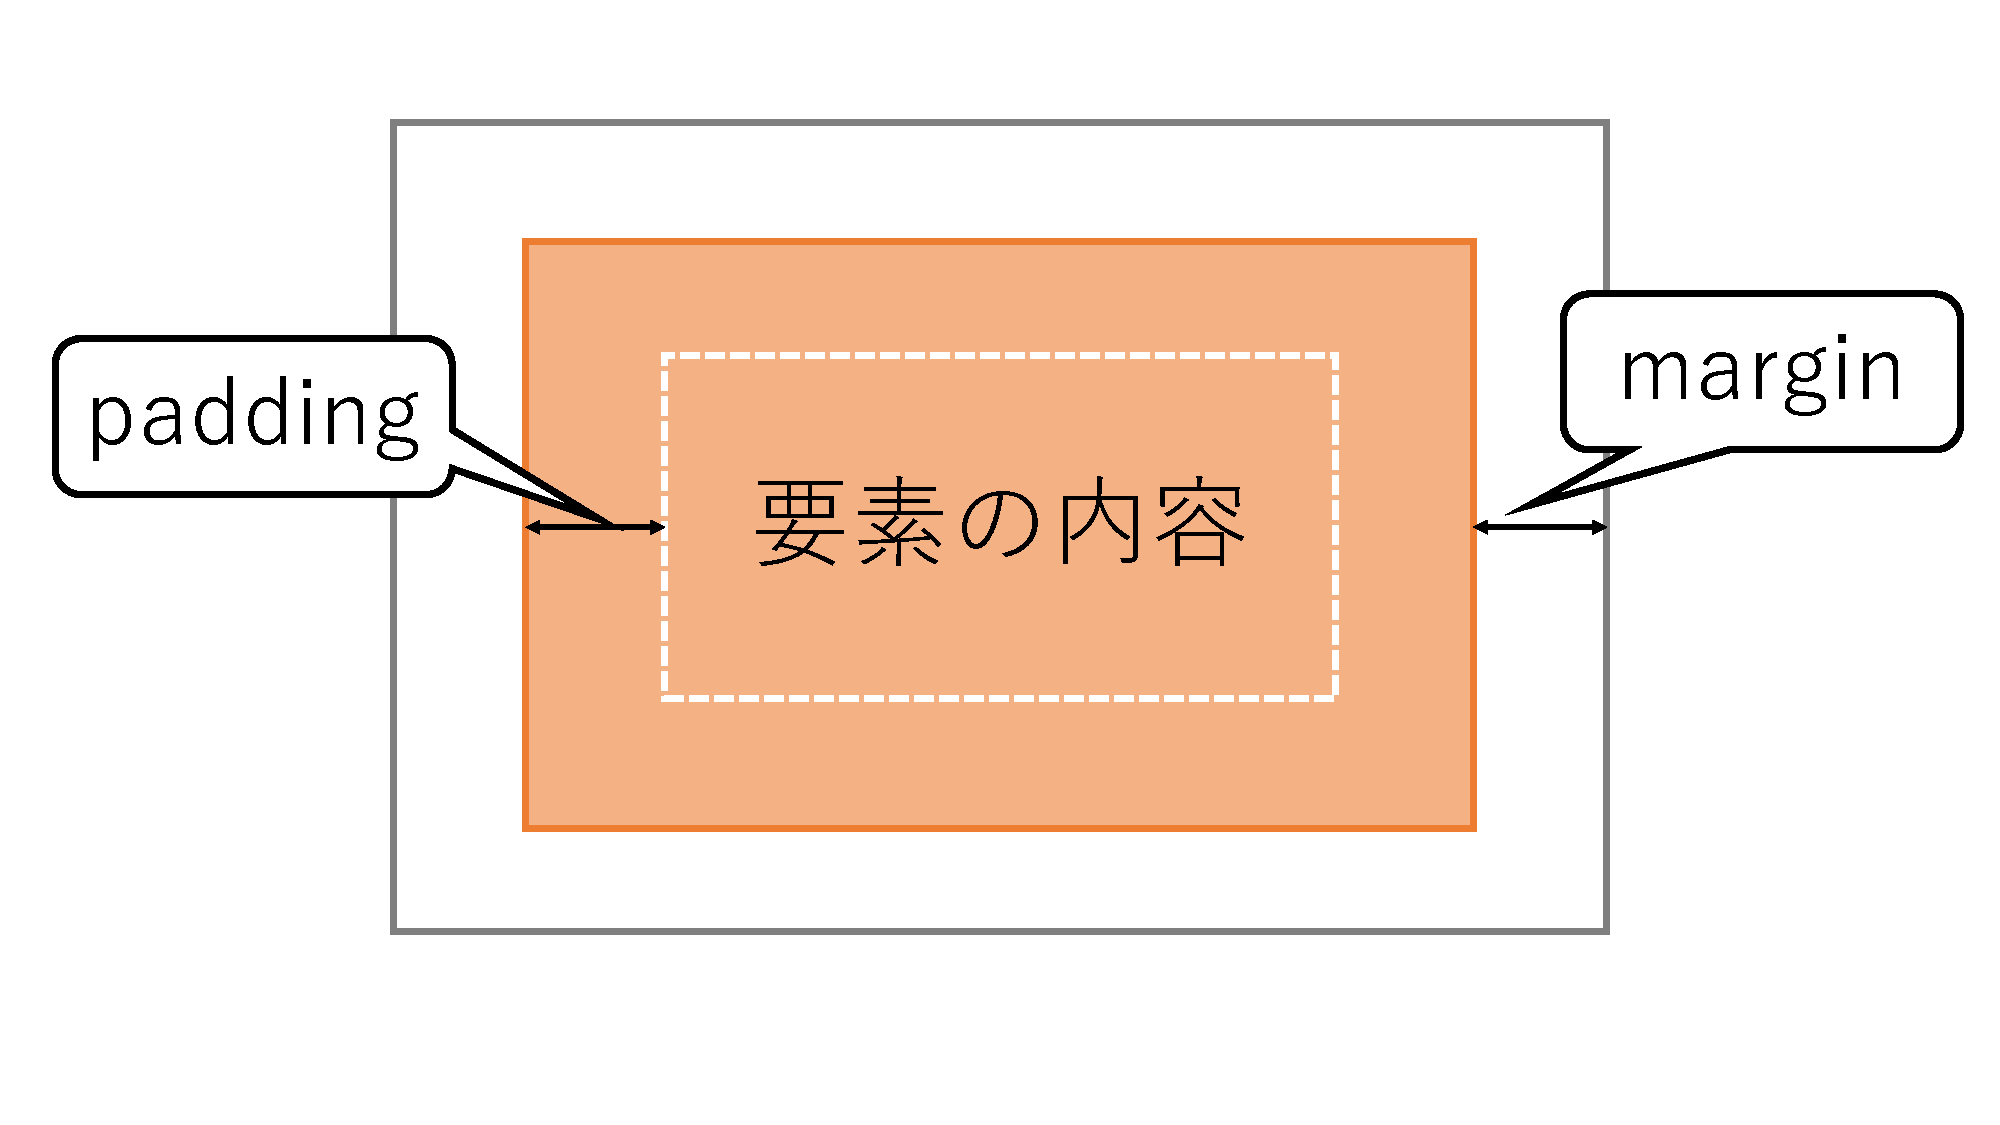
\includegraphics[width=120mm]{./figures/marginpadding.pdf}
 \caption{marginとpaddingのイメージ図}
 \label{fig:marginpadding}
\end{figure}

displayは要素の並べ方を表す.
値は様々なものがありここではblock,inline,inline-block,flexを例として示す.
inlineは幅と高さを指定できなくて余白は左右しかできないが,要素の配置を指定できるといった特徴がある.
blockは幅と高さ,余白を自由に調整できるが,要素の配置を指定できないといった特徴がある.
inline-blockは,幅と高さ,余白を自由に調整でき,要素の配置も指定できるといった特徴がある.
flexは,要素を横に並ばせられるといった特徴がある.

\begin{table}[h]
  \centering
  \caption{CSSのプロパティの例}
  \label{table:css}
  \small
  \begin{tabular}{cc}
    \hline
    プロパティ  & 説明    \\
    \hline \hline
    width  & 横の長さ\\
    \hline
    height  & 縦の長さ\\
    \hline
    margin  & 要素の内容の外側の余白 \\
    \hline
    padding  &  要素の内容の内側の余白\\
    \hline
    display  &  要素の並べ方\\
    \hline
    text-align  &  文字や画像の揃え方\\
    \hline
    position  &  要素の位置の決め方\\
    \hline
    transform  &  要素の動き\\
    \hline
  \end{tabular}
\end{table}

\newpage
\section{結言}
音楽制作には, 作曲,作詞,編曲のほかに,複数の音源をエフェクターを用いて整え一つにする「ミックスダウン」という工程がある\cite{mix}.
近年は,コンピュータ上で音楽制作ができるDTMが普及して手軽に音楽制作ができるようになった.
また,近年のデジタル化により,機材がハードウェアからソフトウェアになり,ミックスダウンも費用をかけずに誰でも挑戦することができるようになった\cite{digital}.

しかし,ミックスダウンは,作曲,作詞,編曲に比べ,変化が分かりにくく,非常に学びづらい.
また, ミックスダウンの経験が少なく,エフェクターを使いこなせない人にとってが説明だけではわからないという問題点がある。

本研究では, 実際に操作をすることで, 各エフェクターの使い方やその効果を知るためのシミュレータ教材を開発した.
このシミュレータを使い,実際に体感することで,エフェクターの効果と変化の理解ができることが期待される.
また,今後はこのシミュレータに効果があるのかを実際に使ってもらい,評価していきたい.

\newpage
\section{謝辞}
本研究の遂行及び本論文の作成にあたり,須田研究室の仲間と制作にご協力いただいた皆様に深く感謝の意を表します.
そして,何よりも本論文の作成にあたり,多大なる御指導及び御助言を頂きました須田宇宙准教授に深く感謝の意を表します.

\newpage
%参考文献
\begin{thebibliography}{99}
\bibitem{mix} ミックスダウンとは?その目的と作業内容、マスタリングとの違いを解説! OTO×NOMA, \url{https://kensukeinage.com/whats_mix/}, 2022/8/21参照
\bibitem{digital} CDの「デジタル・リマスタリング」ってなんだ?|テクの雑学|TDK Techno Magazine, \url{https://www.tdk.com/ja/tech-mag/knowledge/062}, 2022/8/21参照
\bibitem{history} 音楽の歴史, \url{http://relaxbach.sakura.ne.jp/ongaku/rekisi.html}, 2022/12/30参照
\bibitem{dtm} DTM初心者・入門者にオススメ!|DTM初めてガイド【DTMとは?パソコンの種類と必要機材】|島村楽器オンラインストア, \url{https://store.shimamura.co.jp/ec/contents/ols/00dtm/vol1.html}, 2022/12/20参照
\bibitem{daw} DTMとは?DAWとは? | Rock oN Company | DTM DAW 音響機器, \url{https://www.miroc.co.jp/how_to/dtm/}, 2022/12/20参照
\bibitem{software} ソフトウェア音源とは? - DAW.COM, \url{https://dawcom.wiki.fc2.com/wiki/ソフトウェア音源とは?}, 2022/12/30参照
\bibitem{html} HTMLとは?簡単なHTMLタグの基本からCSSの基礎まで初心者にもわかりやすく解説 | MarkeTRUNK, \url{https://www.profuture.co.jp/mk/column/20024}, 2023/1/3参照
\bibitem{html5} 必ず覚えておきたいHTML5の特徴と新機能/HTML5完全読本\#1-1 | HTML5完全読本―実践テクニックとWebデザインの最新動向 | Web担当者Forum, \url{https://webtan.impress.co.jp/e/2014/04/24/17355}, 2023/1/3参照
\bibitem{api} JavaScriptでAPIを呼び出す方法を現役エンジニアが解説【初心者向け】 | TechAcademyマガジン, \url{https://magazine.techacademy.jp/magazine/19615}, 2023/1/8参照
\bibitem{css} CSSとは?-CSSの基本, \url{http://www.htmq.com/csskihon/001.shtml}, 2023/1/8参照
\end{thebibliography}

\newpage

\section*{付録}
\lstinputlisting[caption = EQ.js ,label = js]{EQ.js}
\lstinputlisting[caption = EQ.html ,label = html]{EQ.html}

\end{document}
